\documentclass[pdftex,12pt,a4paper]{report}

\usepackage{a4wide}
\usepackage{setspace}
\onehalfspace

\usepackage{natbib}
\bibliographystyle{agsm}
\renewcommand{\bibsection}{\appendix\chapter{\refname}}

\usepackage{url}
% I'm not completely sure what this does...
% http://tex.stackexchange.com/questions/9445/urls-break-compilation
\renewcommand{\harvardurl}[1]{\textbf{URL:} \url{#1}}

\usepackage{graphicx}
\usepackage{wrapfig}
\usepackage{tikz}
\usepackage{todonotes}
\usepackage{mathtools}
\usepackage{amssymb}
\usepackage{booktabs}
\usepackage{pdfpages}
\usepackage{pgfplots}
\pgfplotsset{compat=1.3}

\usepackage{listings}
\lstset{basicstyle=\footnotesize\ttfamily\singlespacing,frame=single}

\usepackage{titlesec}
\titleformat{\chapter}[display]{\normalfont\huge\bfseries\raggedright}{\chaptertitlename\ \thechapter}{20pt}{\Huge}
\titlespacing*{\chapter}{0pt}{50pt}{40pt}

\newcommand{\HRule}{\rule{\linewidth}{0.5mm}}

\usepackage{epstopdf}

\begin{document}
\begin{titlepage}
\begin{center}

~
\vspace{3cm}

Submitted for the degree of B.Sc. in Computer Science, 2012\\[0.5cm]

% Title
\HRule \\[0.4cm]

{ \huge \bfseries Augmenting a Monte Carlo Tree Search Agent for Ms Pac-Man with Machine Learning Techniques}\\[0.4cm]

\HRule \\[1.5cm]

\begin{minipage}{0.4\textwidth}
\begin{flushleft} \large
\emph{Author:}\\
Stewart \textsc{MacKenzie-Leigh}\\
200714763
\end{flushleft}
\end{minipage}
\begin{minipage}{0.4\textwidth}
\begin{flushright} \large
\emph{Supervisor:} \\
Dr.~John \textsc{Levine}
\end{flushright}
\end{minipage} \\[2cm]

\end{center}

"Except where explicitly stated all the work in this report, including appendices, is my own and was carried out during my final year. It has not been submitted for assessment in any other context."\\

"I agree to this material being made available in whole or in part to benefit the education of future students." \\[0.5cm]

\begin{flushleft}
Signed: \\[0.5cm]
Date:
\end{flushleft}

\end{titlepage}


\thispagestyle{empty}
\mbox{}
\newpage

\chapter*{Acknowledgements}

I would like to thank my supervisor Dr John Levine for his guidance throughout this project.  Thank you also to Phil Rogers for his help and support.

Finally I am grateful for the moral support from my friends and family during my studies.


\thispagestyle{empty}
\mbox{}
\newpage

\begin{abstract}
\end{abstract}


\thispagestyle{empty}
\mbox{}
\newpage

\pagenumbering{roman}
\tableofcontents
\listoffigures
\listoftables

\pagenumbering{arabic}

\chapter{Introduction}
\label{ch:intro}

\chapter{Related work}
\label{ch:related}


\section{The Ms~Pac-Man environment}
The original Pac-Man was an arcade game developed by Toru Iwatani, a Japanese games designer working for Namco Company, in 1980~\citep{Samothrakis2011}.  It became hugely successful due to its wide appeal and a number of spin-offs were created.  One of these was Ms~Pac-Man, which was initially created unofficially before being sold to Midway Games, who distributed Namco games in North America.

The original game features a pizza-shaped protagonist ``Pac-Man'' which the player must direct around a maze consuming ``pills'' and occasionally fruit when it becomes available, whilst avoiding the four ghosts (``Pinky'', ``Inky'', ``Blinky'' and ``Clyde'') which attempt to eat Pac-Man.  If they succeed, Pac-Man loses a life.  There are four ``power pills'' in the maze: if Pac-Man eats one, all the ghosts turn blue and become edible.  Eating as many ghosts as possible in this state confers a significant advantage, as not only is the player rewarded with a number of points upon eating a ghost, the number of points on offer for a ghost doubles with each one eaten.  Starting at 200 for the first ghost, it increases to 400, 800, and 1600 for each consecutive ghost eaten whilst the same power pill is still active.  Thus, the total score available from a power pill is 3050 (50 for the power pill itself, and the sum of the scores mentioned above)---this is in contrast to only 10 points for each regular pill consumed.  Once all the pills in a maze have been cleared, the next level is reached.  Ghosts stay edible for decreasing amounts of time in each subsequent level, making it harder both to score points and to stay alive.

The original Pac-Man featured deterministic ghost behaviour and so it is possible to exploit known patterns of behaviour to learn how to play a given level in such a way that the maximum score for that level is always achieved.  However, Ms~Pac-Man features more sophisticated ghost behaviour which involves a level of non-determinism, making it much more difficult to play.  The other notable difference between the two games is that the latter has four levels instead of just one; there are other minor cosmetic differences such as the renaming of the orange ghost previously known as ``Clyde'' to ``Sue'', and the addition of a red bow and lipstick to the Pac-Man character.

Ms~Pac-Man is now more than thirty years old, a considerable time in the technology arena, and much more sophisticated games exist for the exponentially faster hardware available today; however, it remains useful to artificial intelligence research.  Much work has been done in creating game-playing agents for a wide range of games including chess, checkers, Go, and even Jeopardy, and these agents are often at least as good as human champions.  However, the task environment \todo{Read Russell and Norvig} of Ms~Pac-Man presents several interesting challenges.

Unlike the games mentioned above, the Ms~Pac-Man environment is \emph{dynamic} rather than \emph{static}: whilst in chess the state of the game remains fixed between moves, the state in Ms~Pac-Man is continuously changing, even if the agent is not making any moves.  Additionally, rather than being afforded several minutes to deliberate, the agent must post a move relatively frequently (every 40~ms in the framework mentioned below).  Thus, the environment is also \emph{quasi-continuous} as opposed to being completely \emph{discrete} like board games.

Board games also tend overwhelmingly to be \emph{deterministic}, meaning that the results of a move can be completely and exactly determined by the agent.  In contrast, the Ms~Pac-Man environment is \emph{stochastic}: the ghosts incorporate random behaviour and therefore cannot be completely predicted.  Further complicating the problem of predicting the state of the game after a move is the fact that both Ms~Pac-Man and the ghosts make moves \emph{simultaneously} rather than taking turns as in the majority of board games.

However, the player does have knowledge of the whole game state available to them when making a decision, an attribute shared with traditional board games.  Similarly, all actions available to the player in a given state can be fully known and enumerated.

It can be seen that although Ms~Pac-Man is a seemingly simple, having a trivial objective and few rules, it is perhaps deceptively so, and certain aspects of the task environment greatly increase the complexity of developing an effective agent.  Accordingly, the performance of artificial agents falls somewhat short of the scores achieved by human players.

The usefulness of Ms~Pac-Man to the field of artificial intelligence has previously been recognised and there exists a reasonable amount of research on the subject to date.  This has been encouraged by the creation of various frameworks and competitions to facilitate the development of artificial agents.  The original code is closed source and not designed to run on modern computers, and thus frameworks have had to be written to enable custom agent code to interface with the game.  Various authors~\citep{Lucas2005,Koza1992} have implemented their own simulated versions of the game, sometimes with quite different behaviour to the original game. \citet{Robles2009} also implemented their own version, as well as providing a framework which uses a screen capturing technique to allow the agent to extract information out of the original game running in an emulator.  They demonstrated that their simulator framework and the screen capture framework were roughly equivalent.

It is argued that exact equivalence to the real game is not important however, as the main motivation of such research is not necessarily to write an agent capable of playing the real game well (on its own, a goal of somewhat questionable utility); rather it is to write an agent capable of dealing with the kind of complexities inherent in a game such as Ms~Pac-Man.  As long as the simulated task environment is not significantly different to the real one as described above, the same benefits may be derived from the research.  It is nevertheless important to note that scores obtained by agents under different simulators cannot readily be compared.

The framework used in this work, the aforementioned simulator framework, was developed at the University of Essex~\citep{Robles2009} and used to host various competitions such as at the 2009 IEEE Conference on Computational Intelligence and Games (CIG 2012\footnote{\url{http://geneura.ugr.es/cig2012/}}) and at the IEEE World Congress on Computational Intelligence (WCCI 2012\footnote{\url{http://www.ieee-wcci2012.org/}}).  The framework is written in Java and closely replicates the original game, with a few notable exceptions:

\begin{itemize}
\item Ms~Pac-Man and the ghosts travel at the same speed, unless a power-pill is active, in which case Ms~Pac-Man can move faster than the ghosts.  Unlike the original, Ms~Pac-Man does not slow down when eating pills.
\item In the original, ghosts slow down in the ``tunnels'' at the side of the screen, providing an opportunity to put some distance between Ms~Pac-Man and a pursuing ghost.  This is not the case in the simulator.
\item The simulator does not include the bonus fruit.
\item The behaviour of the ghosts can be determined by any custom ghost controller class.  This is a significant difference which makes the task not only much harder, but arguably much more interesting, as tactics which are effective against one ghost ``team'' may not be effective against another.  The competitions generally feature user-submitted ghost teams as well as Ms~Pac-Man controllers and therefore it is not possible to know in advance what ghost teams the agent should be able to play against.  This point is the main reason behind this paper.
\end{itemize}

\section{Monte Carlo tree search}

\subsection{Background in tree search for games}

Traditional tree search algorithms have been successfully applied to numerous board games such as chess and checkers.  However, these algorithms have been found lacking in some areas, as they can be slow to run and require significant domain knowledge to produce effective agents.  More specifically, the \emph{evaluation function} which evaluates the strength of a particular game state has proven particularly difficult to write for many games.

One such game is Go \footnote{see \url{http://www.gobase.org} for an introduction}.  Chess has an 8~$\times$~8 board, and it is relatively easy to calculate from a given chess position which player has the upper hand by considering aspects such as material count and position.  On the other hand, the Go board (known as the \emph{Goban}) ranges from 9~$\times$~9 for beginners up to as large as 19~$\times$~19, and even experts disagree on the quality of given game states.  The technique of alpha-beta search \todo{cite Russell and Norvig} has proven very powerful for chess players, but the significantly higher branching factor of the game tree given by the larger board and the inability to write an effective \emph{evaluation function} for game states renders the technique of alpha-beta search ineffective for Go~\citep{Gelly2006}.

The Scrabble player \emph{Maven} was one of the first players to make use of simulated game play~\citep{Sheppard2002}.  The merits of different actions are evaluated by playing simulated games for each action, giving an insight into which move will prove to be the better choice as the game develops.  A similar technique has also been used for poker~\citep{Billings2002} and for backgammon~\citep{Tesauro1996}.  However, these players used uniform sampling of available actions or incorporated an unreliable heuristic, leading to much unnecessary simulation.  The UCT (``UCB applied to Trees'') algorithm~\citep{Kocsis2006} was developed in order to more intelligent chose actions to dedicate simulation time to; this effectively developed into the Monte Carlo tree search algorithm.

\subsection{The Monte Carlo tree search algorithm}

\begin{figure}
\label{fig:MCTS}
\missingfigure{MCTS diagram (Chaslot maybe)}
\end{figure}

Monte Carlo tree search (MCTS) is a best-first search technique in which many simulated games are run in order to build a tree of possible game states~\citep{Chaslot2008}.  Each node in the tree represents a game state after taking a given action, represented by the edge from the previous state to the new state.  The algorithm has the following four phases (illustrated in figure \ref{fig:MCTS}):

\textbf{Selection} ~Starting at the root node, the algorithm moves through the search tree by selecting a child of the current node according to some selection policy.  In order to avoid wasting time simulating games for poor moves, the policy must show a preference for choosing moves which have already demonstrated a good reward in previous simulations: this is known as \emph{exploitation}.  On the other hand, the policy must also choose nodes which have been sampled less, so that they may be further investigated: this is known as \emph{exploration}.  This \emph{exploitation versus exploration} dilemma is also seen in multi-armed bandit problems, for which various algorithms exist~\citep{Auer2002}.  The application of this type of algorithm to the selection phase of MCTS is what makes it useful over traditional Monte Carlo methods, as it dramatically decreases the search space.  The UCT algorithm~\citep{Kocsis2006} mentioned above is one of the most commonly-used algorithms for this.

\textbf{Expansion} ~Once a leaf node is reached, it may be expanded.  Expanding a node only once a certain sample count has been reached can produce better results \todo{Expansion threshold citation}.  If the node is expanded, one of its children should be chosen as the new leaf node: this can be a random decision, as the algorithm has no other information.

\textbf{Simulation} ~Also called \textbf{roll-out}, this phase involves running a simulated game from the game state represented by the leaf node arrived at.  In some of the earlier specifications of the algorithm, it was stated that the simulation should be continued until the end of the game~\citep{Chaslot2008}; however, it can also be run until some fixed point in the future, such as after a certain amount of moves.

\textbf{Backpropagation} ~After the simulated game has completed, the tree should be updated with the results.  This may be a simple win/loss ratio, but can be more complex.  For example, an n-player game may backpropagate a score for each player~\citep{Samothrakis2011}.

MCTS has been successfully applied to Go~\citep{Gelly2006} where it significantly improved upon the performance of existing players based on traditional tree search.  This is in part due to the efficient reduction in search space afforded by the UCT algorithm, and also because MCTS does not need an evaluation function.  Instead, random games are played from a game-state until the end of the game, and the score is backpropagated to the node.  MCTS has also been shown to be effective in nondeterministic games and those with imperfect information~\citep{Kocsis2006}.

As Ms Pac-Man has a high branching factor and is non-deterministic, MCTS is suited to the task.

\section{Previous Ms Pac-Man agents}

One of the earliest known studies into Ms~Pac-Man was conducted by \citet{Koza1992}, using genetic programming \todo{Add details from book. D006.31 KOZ}.

\citet{Gallagher2003} created a simplified version of the game containing only regular pills and one ghost.  The agent has two states:

\begin{itemize}
\item The \emph{explore} state: Pac-Man is further than a predefined distance from the ghost.
\item The \emph{retreat} state: Pac-Man is closer than the predefined distance to the ghost.
\end{itemize}

For each of the states, the agent has a set of parameterised probabilistic rules; the parameters are learned using the population-based incremental learning (PBIL) algorithm.  The agent was able to learn the parameters and showed some success, however the authors note that it may be infeasible to scale their approach up to the full game.

\todo[inline]{Finish related work section}

\citet{Me2012} developed an agent using Monte Carlo tree search as part of an ensemble approach.  Prior to making a decision, any number of registered \emph{evaluators} are allowed to run to modify the results of the MCTS algorithm.  For example, a simple evalutor could spot moves in the game tree which eat power pills when there is already one active, and apply penalties to the scores of those nodes.  Thus, short- and long-range planning components augment the mid-range planning provided by the MCTS algorithm.

Although traditional MCTS utilises random playouts, the agent described in the behaviour uses more intelligent agents to control the playout behaviour, as this was found to have better results.  The paper explores two cases: the case where the model of the ghost behaviour used in the playouts matches the actual ghost controller being played against, and the case where the controllers differ.  In the former, three out of the four evaluator configurations considered were found to improve the score by a statistically significant amount, whilst the latter showed a significant improvement for only one evaluator.  Over all, the scores for the accurate model case were in the region of 50,000-60,000, a great deal more than the 10,000-15,000 achieved by the inaccurate model.

Clearly accurate domain knowledge improves the performance of the agent.  If the controller used during the playouts could adapt its behaviour based on observations of the controller being played against, one could reasonably expect the agent performance to steadily improve as the simulation model starts to more closely match the opponent controller.  This is the essence of this project.

\section{Neural networks}

Neural networks are modelled after the nervous system in humans and animals.  This is composed of (in humans, many billions of) cells called \emph{neurons}.  A wide variety of morphologies exist, but the majority of neurons consist of the same three parts: the \emph{dendrites}, highly branched structures which receive chemical signals from other nearby neurons; the \emph{cell body}, which contains the processes necessary for cell function; and the \emph{axon}, containing a ``trigger zone'' which generates electrical signals over the length of the axon if the input to the dendrites reaches a certain threshold.  The axon has \emph{axon terminals} at the opposite end to the dendrites and cell body; these transmit chemical messengers into the dendrites of connected neurons in response to an electrical impulse.  Neurons can be seen as \emph{integrators} as their output is a function of the inputs received from the many connected neurons \cite[p. 152]{Vander}.

Artificial neural networks also consist of large numbers of ``neurons''.  In general, these have a high-dimensional input vector and produce an output which is a non-linear \emph{activation} function (often a sigmoid function) of the input vector and some weights vector \cite[p. 1]{Annema1995}.  It can readily be appreciated how this is analogous to the biological system: the input vector represents the many incoming connections to the dendrites, while the ``trigger zone'' and axon terminals are represented by the activation function and its output.

Each element of the input vector is multiplied by a corresponding element in the weights vector before being summed and used as the input to the activation function; thus, the weights vector controls how much each input affects the output of the neuron.  The weights are adjusted in a \emph{training phase}: by using a large number of training examples where the output expected of the neuron is known, the weights can be iteratively modified according to a learning rule which seeks to minimise the error between the actual output of the neuron and the expected output for each training example \cite[p. 1]{Annema1995}.  This is a form of \emph{supervised learning} \todo{read R and N for supervised learning}.

Although the exact mechanism of learning in the brain is not fully understood, it is thought to operate along similar lines.  In the \emph{long-term potentiation} model, the connections between neurons (called \emph{synapses}) increase in effectiveness when heavily used \cite[p. 271]{Vander}, which is similar in function to the weights which govern the connections between artificial neurons changing value.

\todo[inline]{Add something from Rumelhart et al (D153.4 PAR)}

The type of artificial neural network used in this work is the two-layer feed-forward network \cite[p. 4]{Aleksander1995}.  This consists of a layer of neurons called the \emph{hidden layer}, which computes some internal representation of the inputs \cite[p. 135]{Aleksander1995}, and a connected \emph{output layer}, which computes the final result of the neural network as a function of the output from the hidden layer.  The term "feed-forward" refer to the fact that the input is passed first to the hidden layer, and then fed forward to the output layer.  It has been shown that such a network is capable of approximating any function \cite[p. 10]{Annema1995}.

\todo[inline]{Maybe add Kolmogrov's theorem (p. 10 of Annema) and comment from p. 135 of Aleksander et al}

\subsection{Backpropagation algorithm}

The use of a hidden layer introduces a problem---the expected output for the hidden layer is not known, and so some method must exist for propagating the errors from the output layer in order to train the weights in the hidden layer.  The algorithm used for this purpose in this work is the backpropagation algorithm \cite[p. 134-149]{Aleksander1995}.

\chapter{Problem description}
\label{ch:problem}

\section{The current agent}

The Ms Pac-Man vs Ghosts framework provides the base implementation of the game for this project: to implement an agent, it is required to subclass the abstract generic class {\tt Controller} and implement the {\tt getMove} function.  The method takes one parameter, the game state, which it can query to make a decision on what move to make.  The return type of the method is specified by the generic type parameter of the class instance:  Pac-Man controllers must extend {\tt Controller{$\langle$}MOVE{$\rangle$}} as they need only return a single move for Pac-Man, while ghost controllers extend {\tt Controller{$\langle$}EnumMap{$\langle$}GHOST, MOVE{$\rangle\rangle$}}, as they must return a mapping of ghosts to moves.

The framework calls the {\tt getMove} method every 40~ms; if the method takes longer than that time to run, its return value is discarded and the last move returned by the function is selected.  Thus, the method has a strict requirement on running time.

\citet{Me2012} implemented an agent which used Monte Carlo tree search.  It makes use of a class called {\tt MonteCarloPacManSimulator} (henceforth referred to as the simulator class) which runs simulated games and builds a game tree representation using MCTS.  The agent repeatedly calls on the simulator class to run iterations of MCTS while there is still time remaining.  Once near the deadline, no more simulations are performed: if the agent is at a decision point, i.e., a junction, wall or power pill, the best move found by the MCTS is returned; otherwise, the {\tt NEUTRAL} move is returned, instructing the character to continue in the same direction as before.  The tree is only reset if a move is made, allowing the agent to build on the previous simulations each game tick, increasing the deliberation time.

MCTS works by using simulated ``roll outs'' of game play.  To do this, the simulator class copies the game state and then repeatedly advances it using particular ghost and Pac-Man controllers until some predefined point (e.g. loss of life, change of level, or after a certain amount of time has elapsed).  The agent was written using a highly modular approach, allowing different implementations to be supplied for various aspects, including the ghost controller to use during simulated playouts.  As discussed in chapter \ref{ch:related}, the final score achieved is an order of magnitude better when the ghost controller used during simulations matches the actual opponent.

\section{Proposed additions to the agent}

The idea behind this work is that if the ghost controller used during playouts could somehow learn to better emulate the observed behaviour of the actual opponent during gameplay, it could result in a better final score.  There are various ways that the ghost controller could learn, and these are discussed briefly below.

\begin{figure}
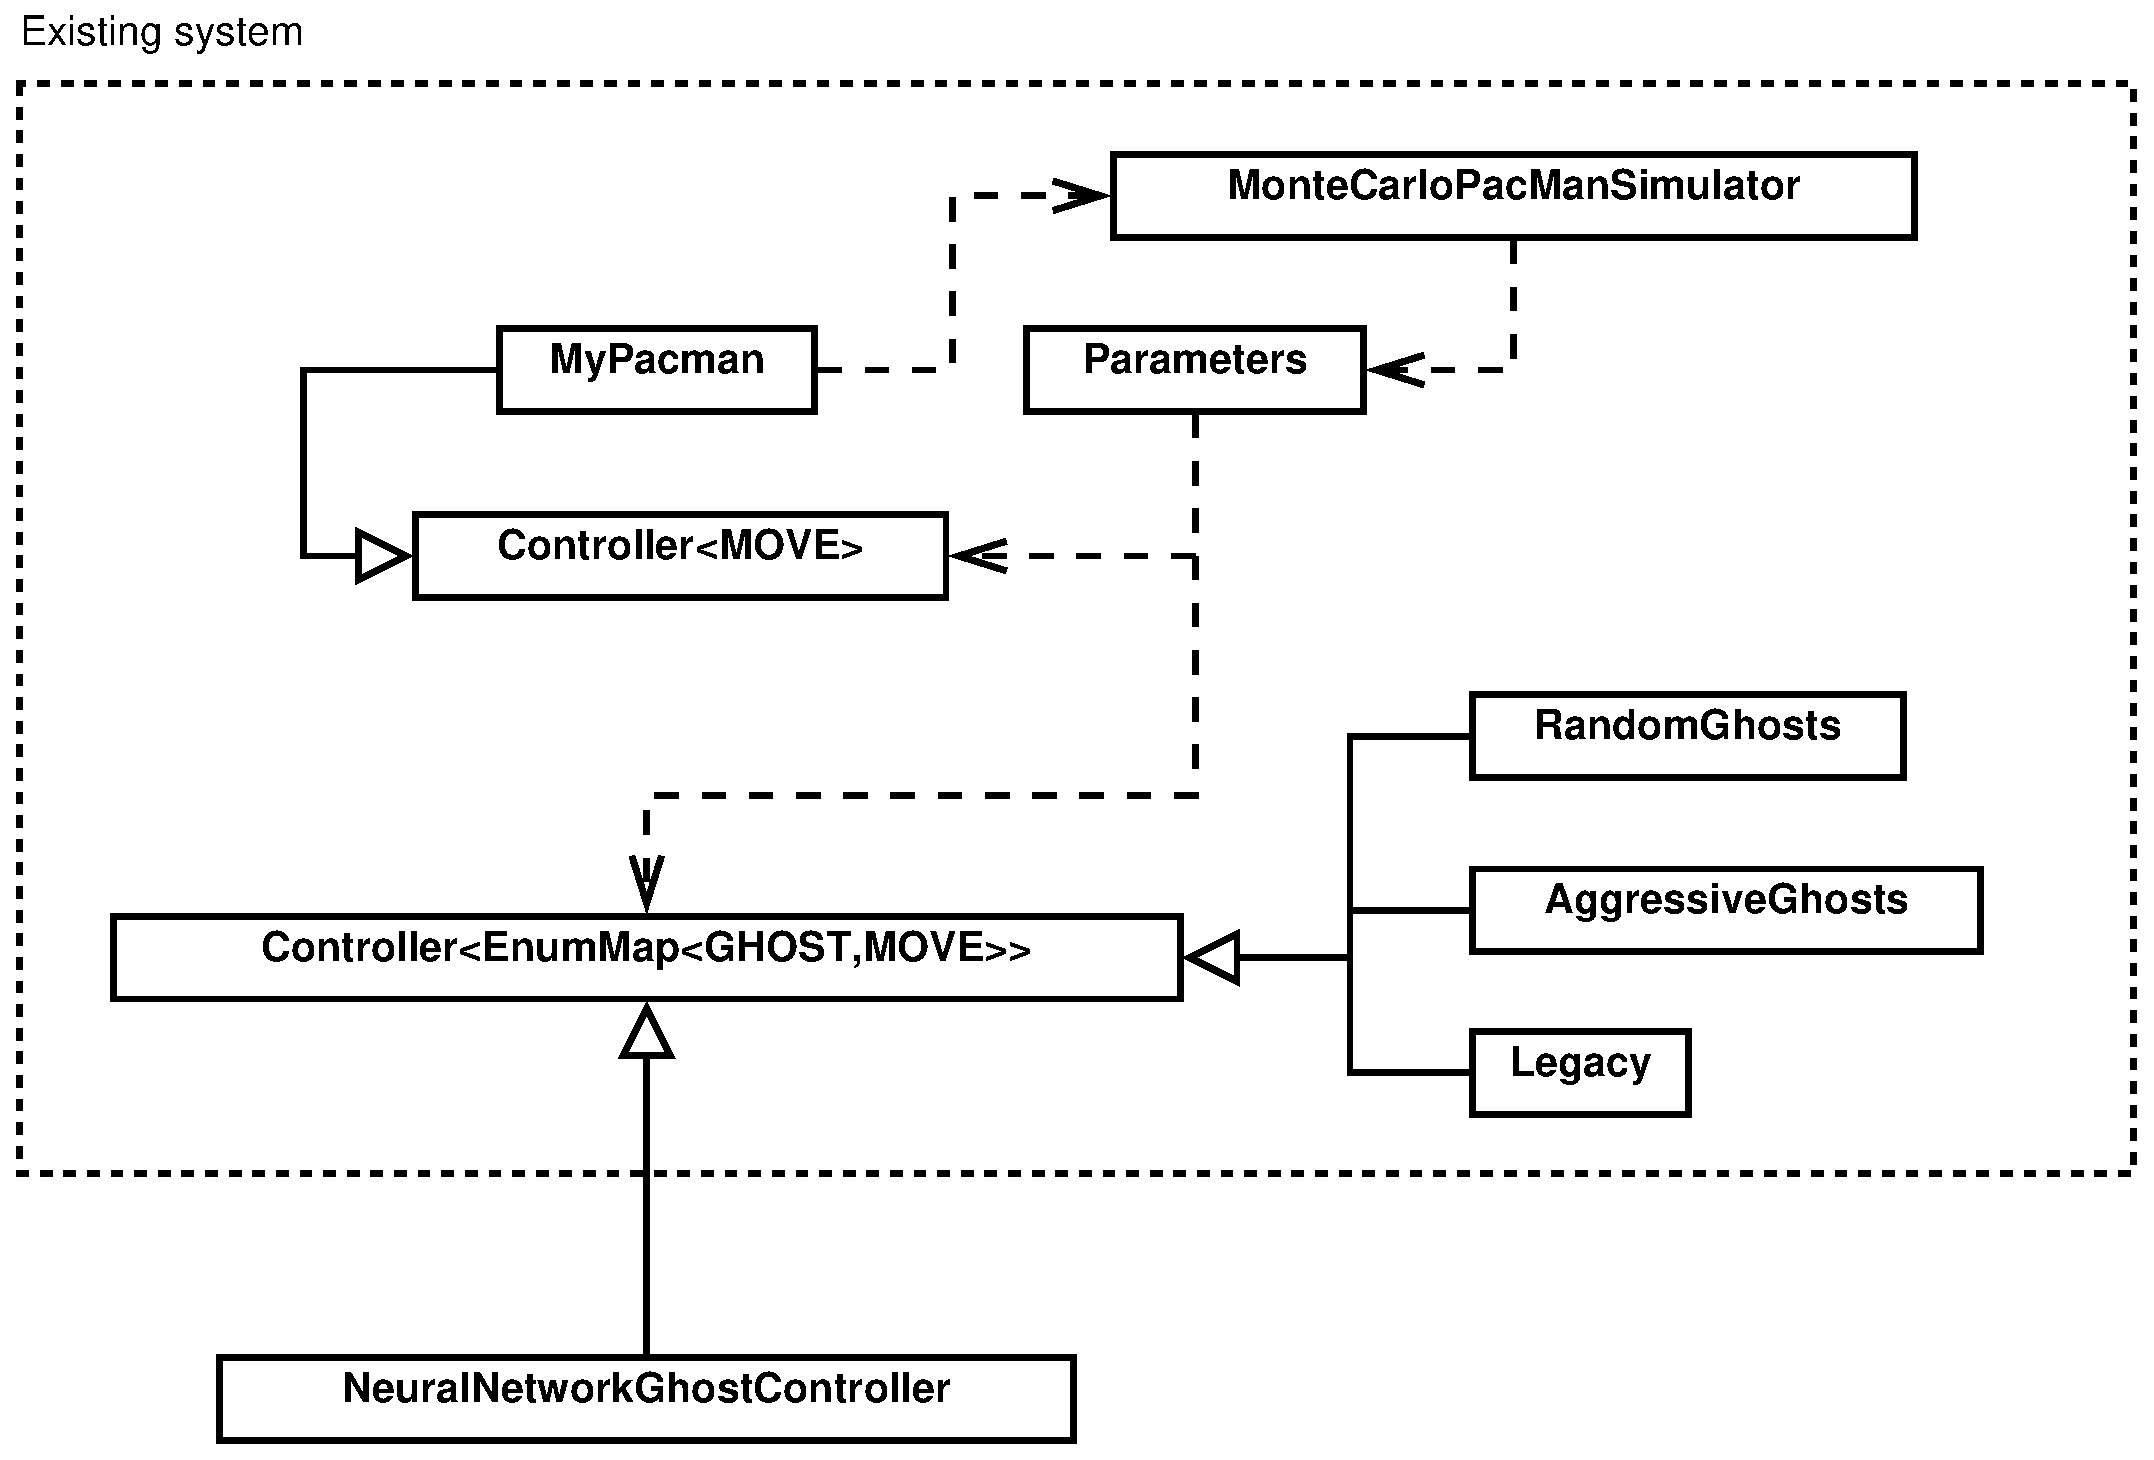
\includegraphics[width=\linewidth]{diagrams/proposed}
\caption[Structural overview]{Structural overview: to implement a Ms Pac-Man agent in the framework, a class extending {\tt Controller<MOVE>} must be created (and it must be called {\tt MyPacman} to be used in the competition).  The existing agent adopts a modular approach: the {\tt Parameters} class contains several fields which specify the behaviour of the algorithm, including one which specifies which ghost controller to use during playouts.  Ghost controllers extend the {\tt Controller<EnumMap<GHOST, MOVE>>} class: some of the example ghost controllers included in the framework are shown.  The proposed addition to the existing agent is a new ghost controller class.}
\label{fig:proposed}
\end{figure}

\subsection{Classifying the ghost behaviour}

One of the first approaches considered at the beginning of this project was to record lots of game data using different opponent ghost controllers, and train a classification algorithm to recognise different kinds of ghost behaviour.  Then during gameplay, the agent could attempt to classify the behaviour observed to determine the known ghost controller which best matches this behaviour, and use this as the controller during playouts.  This has the advantage that a simple classification algorithm, such as logistical regression, is reasonably straightforward to implement.  The downside is that possible opponents in the Ms Pac-Man vs Ghost competitions are extremely diverse, and may not match any of the `known' models.  It would have been interesting to further explore this method if time had available, and it remains a possible opportunity for future work.

\subsection{Reinforcement learning}

\todo[inline]{Reinforcement learning section.}

\subsection{Neural networks}

A neural network is capable of learning behaviour from observed examples, so this seemed like a logical avenue of exploration, and is the method chosen for this project.  Each game tick, the game state is recorded; the following tick, it is possible to retrieve the decisions made on that state for each of the ghosts which needed to make a decision.  This input and observed output is used to train the neural network.

During playouts, the ghost controller uses a neural network for each ghost to decide what moves to return: it feeds as input the elements of game state used during training, and feeds this forward through the network.  Since the network has been trained on the observed behaviour of the opponent, the output of the network should in theory approximate the behaviour of the opponent.

The advantage of this approach is that it should be able to approximate the behaviour of a wide variety of agents.  However, neural network algorithms can be expensive to compute---various optimisations are available but these are often very complex.  Obviously, time spent training the neural network is time that could otherwise be spent on MCTS simulations, so a balance must be maintained.  Furthermore, the agent used during the playouts must feed game state data through the neural networks for each ghost to get predicted moves every simulation tick: this is significantly slower than using a random player and further reduces the amount of simulations that can be run.  A further issue is that a ghost only makes 100-200 decisions in a typical game, and this might not be enough data to train the network particularly quickly.

Finally, at the start of the game before the networks have learnt anything, the ghost controller will effectively be random.  This is not a particularly good choice, and the agent may end up losing all its lives before getting a chance to learn anything.  However, a possible solution to this could be feeding the networks with weights learnt offline on an example controller, so that it is producing at least semi-sensible output even at the start of the game.

\subsection{Requirements}

This discussion draws out a number of requirements.  The addition to the existing agent must perform two functions:

\begin{itemize}
\item Implement a ghost controller which decides on moves player for each ghost, given a game state, using neural networks.
\item Record the decisions of the opponent controller and the game states they were based on each game tick, and use this data to train the neural networks in the ghost controller.
\end{itemize}

Furthermore, the implementation must be fast if it is to be successful.  However, due to the time constraints on the project it may not be possible to implement some of the more advanced algorithms, so a competing requirement is that the implementation must also be reasonably straightforward.

\todo[inline]{Relation to original submitted plan}

\chapter{System design}
\label{ch:design}

\section{Neural network algorithm}
\label{sec:nnalgorithm}
The neural network structure used in the project is a two layer feed-forward neural network \citep[p. 7]{Annema1995}.  The two-layer network features a hidden layer, that is, a layer which is not connected directly to either the input or the output.  It is this feature which gives it the ability to solve ``hard'' learning problems \citep[p. 134]{Aleksander1995}.

However, since the purpose of the hidden layer is to form ``internal representations'' of the data, it is not possible to know what the output of the hidden units should be for a given input.  Therefore, the method of training the network and adjusting the weights of the neurons must be based only on the state of the inputs and outputs to the network, and not of the hidden units \cite[p. 136]{Aleksander1995}.  Backpropagation, discussed in the next section, is one such method of training.

\subsection{Backpropagation}

Much of the theory and the formulae in this section are taken from \citet{Aleksander1995}, chapter 8.  This in turn draws heavily from \citet{Rumelhart1986}, which is much more heavily theoretical and features rigorous proofs of the material presented here; no attempt will be made to replicate this rigour.  Although exactly equivalent, the network here is represented slightly differently and affected formulae are amended accordingly.

\begin{figure}[ht]
\centering
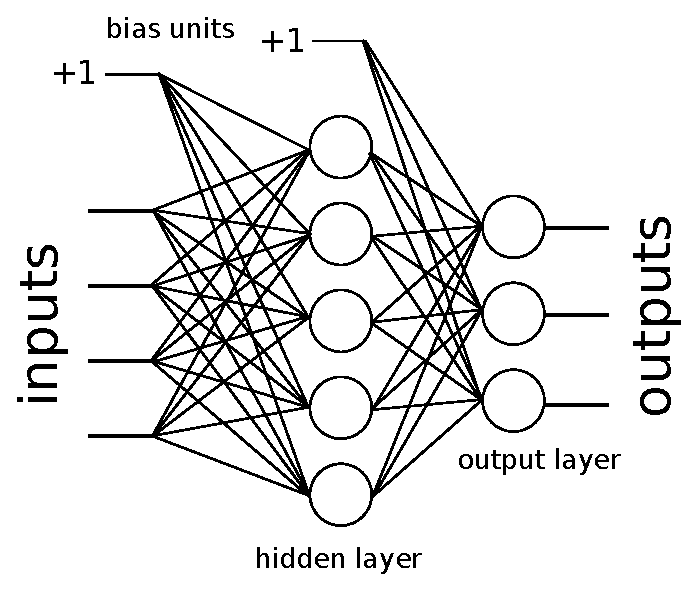
\includegraphics[width=0.5\textwidth]{diagrams/neuralnet}
\caption{A two layer feed-forward neural network}
\label{fig:neuralnet}
\end{figure}

The network topology used is shown in figure \ref{fig:neuralnet}.  It consists of two layers of neurons: the input of every neuron in the first layer (the ``hidden layer'') is connected to every input of the network, and the input of every neuron in the second layer (the ``output layer'') is connected to every output of the first layer.  Finally, the output of the network is defined by the output of the second layer.  The connections between neurons, and betwen inputs and neurons, are each associated with some weight.

Note that some textbooks describe the network as having three layers, the first being the ``input layer'': this description is avoided here, as the inputs are not processed before reaching the hidden layer, i.e., there are no neurons as such in the ``input layer''.

Notice also the two ``bias units'': if the output of each neuron is to compute some aribtrary function of the inputs, they must be able to incorporate some constant value in the function.   \citet{Aleksander1995} describe a \emph{threshold value} which serves the same purpose.  Although a separate threshold value is clearer when dealing with the theory, it will be seen later on that by treating it as a neuron or input which always gives the value 1, the implementation is simplified somewhat.

The \emph{activation} of the $j$th neuron for the $p$th training example, $a_{pj}$, is given by taking the sum for all inputs $i$ multiplied by the corresponding weight, $w_{ji}$.

\begin{equation}
a_{pj} = \sum_{(for~all~i)} w_{ji}o_{pi} + u_j
\label{eq:activation}
\end{equation}

Recalling figure \ref{fig:neuron}, the output $o_{pj}$ of a neuron is the result of some function applied to the activation (equation (\ref{eq:output})).  This function is generally a sigmoid function, and a convenient function to use is shown in equation (\ref{eq:sigmoid}).  It is convenient as its derivative is trivial to determine, and this is required later in the algorithm.  Another popular activation function is $atan(x)$.

\begin{equation}
o_{pj} = f_j(a_{pj})
\label{eq:output}
\end{equation}

\begin{equation}
f(x) = {1 \over 1 + e^{-x}}
\label{eq:sigmoid}
\end{equation}

Using the equations so far, the output of the network can be determined for a given input: first, the outputs of all the neurons in the hidden layer are calculated from the inputs to the neural network; then, the output of the final layer can be calculated from the output of the hidden layer.  It is this process that gives the structure the name ``feed-forward''.

Training the network involves presenting a training example to the network and calculating the output for it using the feed-forward process.  This will give an output, which in the case of a network with no previous training, will be much different from the expected output given by the training data.  The weights are updated as described below to correct for this error, and the training continues.  After many iterations and training examples, the output for a given output will be much closer to the expected value.

Given the $p$th training example, the amount ($\Delta_{p}w_{ji}$) that the weight which joins the $j$th neuron to its $i$th input should be adjusted by is poportional to the calculated error for the unit ($\delta_{pj}$) and a learning rate $\beta$ (equation (\ref{eq:learning})).

\begin{equation}
\Delta_pw_{ji} = \beta\delta_{pj}o_{pi}
\label{eq:learning}
\end{equation}

Calculating the error of output neurons is easy, as the training example states what the expected output is.  The error is therefore the difference between the actual output and the expected output, multiplied by the derivative of the activation function applied to the activation for that neuron (equation (\ref{eq:outputerror})).  Recall the activation function chosen is given by equation (\ref{eq:sigmoid}): its derivative is given by equation (\ref{eq:sigd}).  Note that the value $f(x)$ is the output for the neuron, and has already been calculated by the feed-forward process.

\begin{equation}
\delta_{pj} = (t_{pj} - o_{pj})f'_j(a_{pj})
\label{eq:outputerror}
\end{equation}

\begin{equation}
f'(x) = f(x)\big(1 - f(x)\big)
\label{eq:sigd}
\end{equation}

The errors for the hidden neurons are calculated by propagating the errors back from the output layer, hence the name of the algorithm.  More specifically, the error for the $j$th neuron and the $p$th training example is given by taking the sum of output all errors $k$ multiplied by the corresponding weight $w_{kj}$, all multiplied by the derivative of the activation function applied to the activation for the neuron (equation (\ref{eq:hiddenerror})).

\begin{equation}
\delta_{pj} = \left(\sum_{(for~all~k)}\delta_{pk}w_{kj}\right)f'_{j}(a_{pj})
\label{eq:hiddenerror}
\end{equation}

The described algorithm is a form of gradient descent.  It can be applied to all of the examples in succession, with this being repeated for many iterations; this is called \emph{batch gradient descent}.  As new examples arrive gradually throughout the lifetime of the agent, this project uses the alternative method of \emph{stochastic gradient descent} \citep[p. 720]{RussellNorvig}.

\subsection{Alternatives}

Backpropagation was chosen in this project due to its simplicity and ease of implementation.  Many others have made the same choice, although weaknesses such as slow convergence and a requirement to tune the learning rate are well known.

\citet{Groot1994} showed that algorithms which incorporate higher order information give both a better quality solution (reduced error) and a quicker running time.  By `higher order', the order of the derivatives used by the algorithm is being referred to.  Algorithms which used information from the second derivative of the neural network transfer function were shown to be much more effective.

An exploration of various optimisation algorithms was originally intended as part of this project; however, it turned out to be far too complex to achieve within the time frame.

\section{Proof of concept}

It was necessary to show that it is at least theoretically possible to learn ghost behaviour using neural networks.  First of all, a neural network was implemented in MATLAB; then data from a game was recorded; finally, this data was fed into the neural network implementation to determine if it could be learnt.  The various steps will be described further in the following sections.

\subsection{Neural network implementation in MATLAB}

MATLAB is a mathematical programming language developed by MathWorks.  Although commercial, it is available in many organisations and institutions.  There is also an open source equivalent called Octave: this was initially used, but it lacks several useful functions needed by the project.

One of the benefits of using MATLAB to prototype the neural network is that it can perform operations on variables regardless of whether they represent scalar values or vectors.  For example, in the expression {\tt sin(x)} will return a scalar value if {\tt x} is a scalar, or a matrix of results if {\tt x} is a matrix, using each element in {\tt x} as an input.  Thus, it is convenient if the implementation of the backpropagation algorithm described in section \ref{sec:nnalgorithm} is vectorised.

The inputs to the network are represented as a column vector.  If there are $n$ inputs, there will be $n + 1$ elements in the vector, as the bias unit is added at the top.  If there are $h$ neurons in the hidden layer, the weights which govern the connections between it and the inputs are held in a $h \times (n + 1)$ matrix: for each neuron in the hidden layer, there is a weight to connect it to each of the inputs and the bias unit.  There is a similar matrix for the output layer: in the code, they are called {\tt th1} and {\tt th2} respectively, and they are initially randomly initialised.  This random initialisation is necessary for \emph{symmetery breaking}---if all weight start with the same value, they will always update by the same amount, and the network will be unable to learn anything.

The forward propagation part of the code is given by listing \ref{lst:forward}.  The variable {\tt a1} is the inputs, calculated by taking the $j$th training example and adding the bias unit.  Next {\tt a2}, the hidden layer outputs, is calculated by multiplying the inputs by the weights matrix, applying the activation function\footnote{denoted by the {\tt sig} function, the source code of which is in appendix \ref{ap:matlab}}, and adding the bias unit.  Note that due to the nature of matrix multiplication, the multiply-and-sum operation happens ``for free''.  The output layer is calculated in a similar process, but there is no need to add a bias unit.

\begin{lstlisting}[language=Matlab,label=lst:forward,caption={Forward propagation code},captionpos=b]
a1 = [1; x(j,:)'];
a2 = [1; sig(th1 * a1)];
a3 = sig(th2 * a2);
\end{lstlisting}

After the forward propagation step, backpropagation is performed (listing \ref{lst:backprop}).  The variable {\tt t} represents the target values for the output, and is a vector with a number of elements equal to the number of output nodes.  As described in section \ref{sec:nnalgorithm}, the error of the output nodes ({\tt d3}) is calculated by subtracting the actual output from the target output and multiplying by the derivative of the activation function, defined as {\tt sigd} here.  By using a vectorised implementation, one line of code can perform this function for the whole output layer.

Recall that the error in the hidden layer is given by backpropagating the error from the output layer, using the connecting weights.  The error in the hidden layer is used to calculate the adjustment needed in the weights connecting the hidden layer to the input---since the input is not connected to the bias unit, we do not need to consider it, and that is why the first column (which relates to the bias unit) of {\tt th2} is missed out.

\begin{lstlisting}[language=Matlab,label=lst:backprop,caption={Backpropagation code},captionpos=b]
d3 = (t - a3) .* sigd(a3);
d2 = (th2(:,2:end)' * d3) .* sigd(a2(2:end));
\end{lstlisting}

Now all that remains to be done is to update the weights, shown in listing \ref{lst:update}.  The weights which connect the hidden layer to the input are responsible for any errors resulting in the output of the hidden layer, and the calculated error of the hidden layer is therefore used in updating these weights.  The variable {\tt beta} is the \emph{learning rate}, and governs the rate of gradient descent.  A value of 1 has been found to work adequately.  The weights which govern the connection of the hidden layer and the output layer are updated in a similar fashion.

\begin{lstlisting}[language=Matlab,label=lst:update,caption={Weight update code},captionpos=b]
th1 = th1 + beta * d2 * a1';
th2 = th2 + beta * d3 * a2';
\end{lstlisting}

A full listing of the function described in this section, as well as the listings of the {\tt sig} and {\tt sigd} functions, can be found in appendix \ref{ap:matlab}.  This implementation was verified by ensuring that the network could learn various boolean functions from examples, such as OR, AND, and XOR.  The latter is a `hard' learning problem which can only be learned by multi-layer networks.

\subsection{Logging ghost data}

\subsection{Choosing the neural network parameters}

\subsection{Neural network implementation in Java}


\chapter{Implementation details}
\label{ch:implementation}

\section{Structure}
\ref{sec:structure}

\begin{figure}
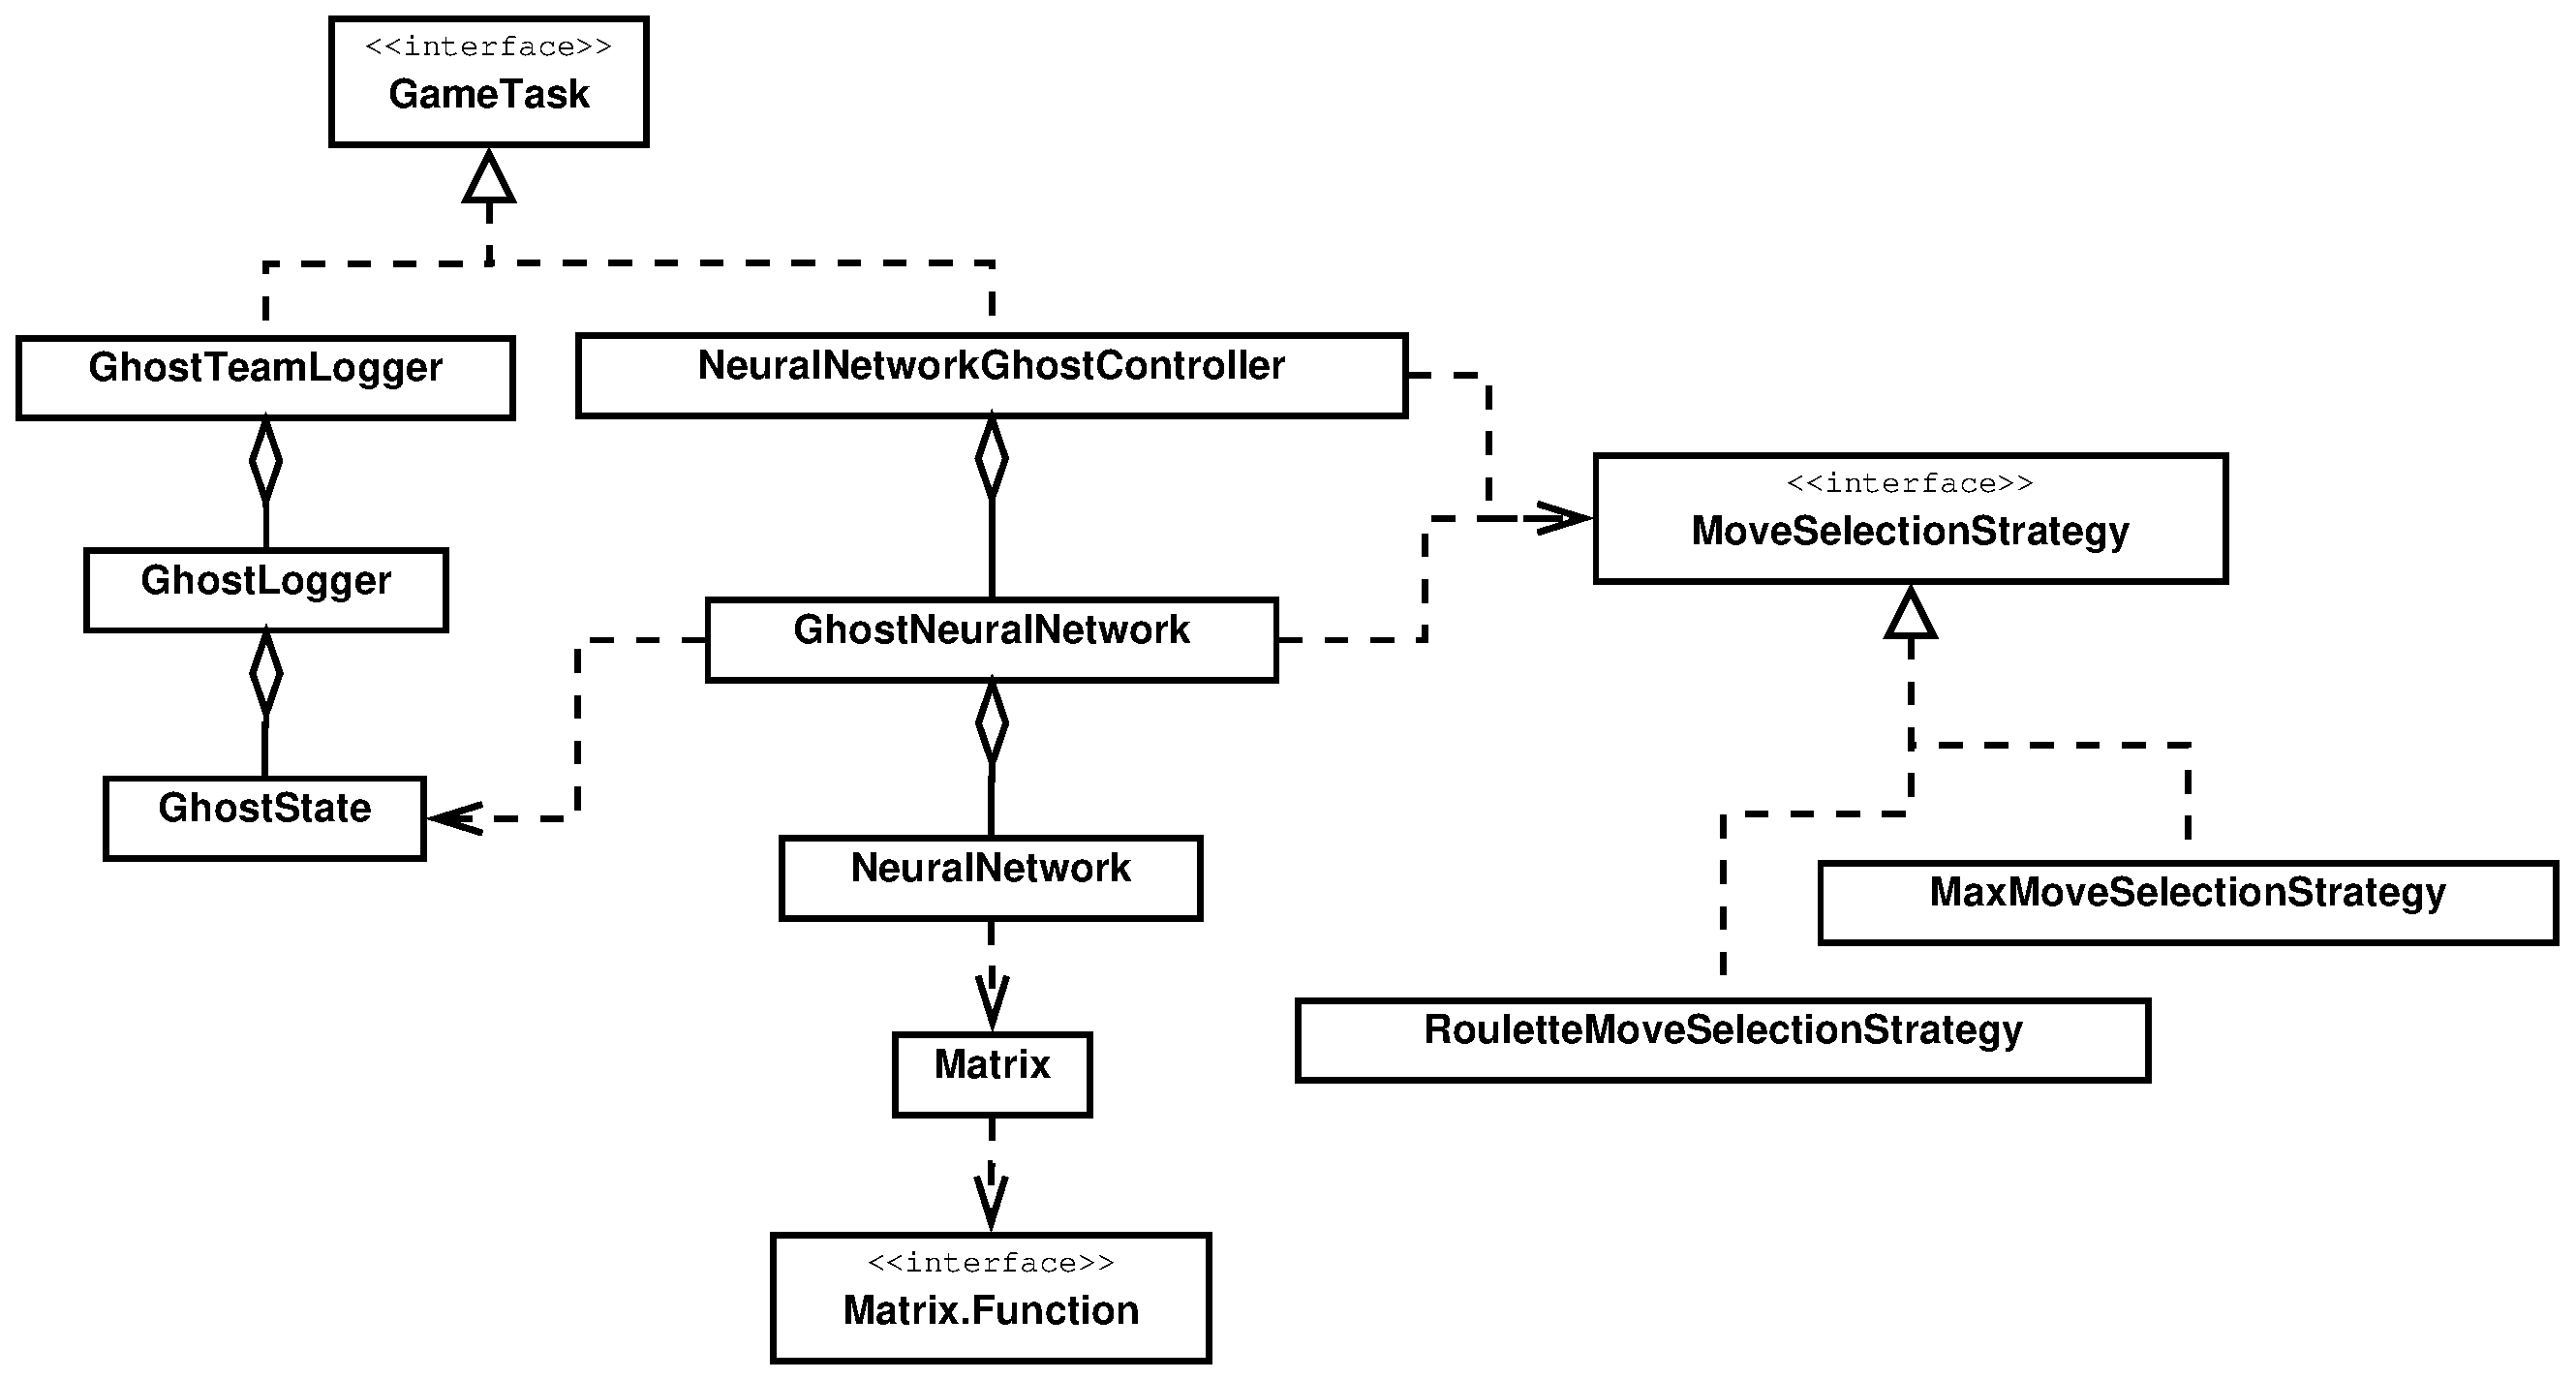
\includegraphics[width=\linewidth]{diagrams/project2}
\caption{Structure of the project}
\label{fig:project}
\end{figure}

Figure \ref{fig:project} shows the overall structure of the project.  The {\tt NeuralNetworkGhostController} class is the main part of the project: this implements the learning ghost controller, and the other classes and interfaces support it.  It uses four instances of the {\tt GhostNeuralNetwork} class, one for each of the ghosts; this class merely wraps the {\tt NeuralNetwork} class to give ghost-specific functionality.  The implementation of the neural network algorithm is in the {\tt NeuralNetwork} class---the chosen method uses matrices (see section \ref{sec:matlab} for more details) and therefore this class depends on the {\tt Matrix} class for matrix operations.  The {\tt Matrix} class is optimised for the specific task, which will be covered in section \ref{sec:efficiency}; this is the reason for not using an off-the-shelf matrix implementation.

The neural network used by each ghost has four real-valued outputs, with each output corresponding to a direction (i.e. up, down, left, right).  There are two ways in which this output could be mapped to a chosen move: the first is to simply find the output with the maximum value (indicating that the network is more ``sure'' about this output) and return the corresponding move; however, since Monte Carlo tree search is a probabilistic algorithm, another method could be to pick the move corresponding to a given output with a probability of the value of the output out of the sum of the outputs, so that the probability of a move being picked is proportional to the certainty the neural network has for that move.  Since there is a choice involved, the \emph{Strategy} design pattern was employed so that different strategies---implementing the {\tt MoveSelectionStrategy} interface---could be chosen at run time.  The former strategy is implemented by the {\tt MaxMoveSelectionStrategy} class, whilst the later is implemented by the {\tt RouletteMoveSelectionStrategy} class.

The input to the neural network is represented by the {\tt GhostState} class.  This class is also used by the {\tt GhostLogger} class to save ghost data to a file for evaluation purposes (see section \ref{sec:logging} for details).  The {\tt GhostTeamLogger} class holds a reference to four instances of this class, one for each ghost, to encapsulate the logging into one class.  It implements the {\tt GameTask} interface which was added to allow classes to be registered to get called every game tick.  The {\tt NeuralNetworkGhostController} class also implements this interface so that it can train each tick.

\section{Matrix efficiency improvements}
\label{sec:efficiency}

Much difficulty was encountered in implementing the neural network in Java.  It was realised that the implementation would have to be efficient, and so it was attempted to write it as such from the start.  However this proved rather difficult as there is much that can go wrong with such a complex implementation, and it is difficult to spot the location of errors: the neural network simply fails to converge and the reason for this is usually not clear at all.

Therefore, the implementation was reattempted with the goal of matching the MATLAB code as closely as possible, with the simplest possible code.  This network was trained using data recorded for Blinky from a game against the {\tt Legacy} controller (containing 1169 data points) in order to demonstrate that it worked.  Then a series of optimisations were made one at a time, each time re-running the test on the same data so that any bugs could be picked up.  This helped localise the source of any problems.  There follows a discussion of the optimisations made with table \ref{tab:optimisations} showing the time saved by each optimisation.  This time was determined by training the network 10 times with the aforementioned data for each optimisation, running for 1000 iterations each time with 10 hidden nodes.  An average was then obtained for each, in order to discount effects such as JVM overhead and temporary demands on the processor.

\subsection{Na\"{i}ve implementation}

The matrix implementation used by the original code used a 2D ``jagged'' array to store the matrix data.  Internally, such an array consists of an array of pointers to a separate array for each row.  Thus to access an element in row 2, column 3 for example (with the code {\tt data[2][3]}) the JVM must find the second element in the main array, dereference the pointer it finds there to get the row array, and then find the third element in that array.

If iterating through the data in a row-major fashion, the Java compiler is not smart enough to store the row array in a temporary variable: doing this manually gives a speed increase.  Iterating in a column-major fashion can actually usurp the efforts of the processor cache if the data is large enough, which greatly hampers the performance.

\begin{lstlisting}[language=java,caption={Multiply code},captionpos=b,label=lst:naive,float]
for (int i = 0; i < op1.rows; i++)
{
    for (int j = 0; j < op2.columns; j++)
    {
        double sum = 0;

        for (int k = 0; k < op2.rows; k++)
        {
            sum += op1.data[i][k] * op2.data[k][j];
        }

        answer[i][j] = sum;
    }
}
\end{lstlisting}

As can be seen from listing \ref{lst:naive}, storing the matrix data like this is the easiest method to understand and therefore the easiest to program correctly; however there is obviously a need to improve the efficiency.

\subsection{An improved representation}

The first optimisation applied was to store the matrix data as a flat array, where each row is stored sequentially.  Thus, instead of accessing {\tt data[2][3]}, the programmer would access {\tt data[2 * numberOfColumns + 3]}.  Multiplication is much slower than repeated adding however, and an even greater saving can be made if adding is used when iterating over the data instead of multiplying.  Note in listing \ref{lst:flatarray} how the indices to each part of the data are stored and multiplication is avoided.

\begin{lstlisting}[language=java,caption={Multiply code with flat arrays},captionpos=b,label=lst:flatarray,float]
int answerindex = 0, op1index = 0, op2index;

for (int i = 0; i < op1.rows; i++)
{
    for (int j = 0; j < op2.columns; j++)
    {
        double sum = 0;
        op2index = j;

        for (int k = 0; k < op2.rows; k++)
        {
            sum += op1.data[op1index + k] * op2.data[op2index];
            op2index += op2.columns;
        }

        answer[answerindex++] = sum;
    }

    op1index += op1.columns;
}
\end{lstlisting}

This is by far the biggest improvement in efficiency out of all the techniques applied, with the time taken to run 1000 iterations on the network dropping from 28.5 to just 12.8---a saving of 15.7 seconds.

\subsection{Further enhancements}

The further enhancements optimise for specific patterns found in the neural network code that uses the matrix implementation (the neural network algorithm can be found in appendix \ref{ap:matlab}).

Firstly, it was realised that many of the multiply operations were performed after first transposing one of the operands.  The transpose operation is quite slow as it involves iterating over the data and copying it to a new location, but it is really only rearranging the data: if instead the multiply function was to iterate over the operand data in such a way that mimicked one of the operands having been transposed, the transpose operation could be skipped entirely.  Therefore, two extra multiply functions were written: one which simulated transposing the first operand, and another which simulated transposing the second operand.  This improvement reduced the time taken by a further 2.7 seconds.

It was also noticed that often in the neural network algorithm, some matrix operation is performed such as multiplication or addition, then some function is applied to all of the elements of the resulting matrix.  The na\"{i}ve implementation has to iterate over all the data twice in this scenario, but a better approach would be to give the ability to apply the function to each element as the first operation is happening.  An interface was made representing an element-wise function, and an argument was added to each of the element operator functions to accept an instance of this interface.  This optimisation reduced the over all time by a fifth of a second.

Other modifications were then made in the same vein, designed to avoid iterating over the data more times than is necessary.  Each step in the algorithm dealing with forward propagation, backward propagation and finally updating of the neural network weights was implemented in a custom function, resulting in the overall running time on the test data being reduced to just under 5 seconds.  This is a significant saving from the original 28.5 seconds.  Listings \ref{lst:before} and \ref{lst:after} show the neural network algorithm before and after optimisations respectively.

\begin{table}[ht]
\centering
\begin{tabular}{lcc}
\toprule
Description & Running time (s) & Saving (s) \\
\midrule
Na\"{i}ve implementation & 28.535 & --- \\
Flat array storage & 12.767 & 15.768 \\
Transpose / multiply shortcut & 10.080 & 2.687 \\
Element-wise function shortcut & 9.875 & 0.205 \\
Custom weights updating & 7.264 & 2.611 \\
Custom forward propagation & 5.254 & 2.010 \\
Custom hidden layer error calculation & 4.966 & 0.288 \\
Custom output error calculation & 4.946 & 0.02 \\
\bottomrule
\end{tabular}
\caption[Algorithm running time after various optimisations]{Algorithm running time after various optimisations: each line follows on from the previous, thus the last line is the cumulative effect of all the previous optimisations.}
\label{tab:optimisations}
\end{table}

\begin{lstlisting}[language=Java,caption={Neural network algorithm before optimisation},label=lst:before,captionpos=b,float]
a1 = Utilities.appendVertical(1, x.part(j, j, 1, -1).transpose());
a2 = Utilities.appendVertical(1, theta1.multiply(a1).apply(sig));
a3 = theta2.multiply(a2).apply(sig);

t = y.part(j, j, 1, -1).transpose();
d3 = t.subtract(a3).elementMultiply(a3.apply(sigd));

d2 = theta2.part(1, -1, 2, -1).transpose().multiply(d3)
		.elementMultiply(a2.part(2, -1, 1, 1).apply(sigd));

theta1 = theta1.add(d2.multiply(a1.transpose()).scale(learningRate));
theta2 = theta2.add(d3.multiply(a2.transpose()).scale(learningRate));
\end{lstlisting}

\begin{lstlisting}[language=Java,caption={Neural network algorithm after optimisation},label=lst:after,captionpos=b,float]
a1 = x.getRowAsColumn(j);
a2 = calculateLayer(theta1, a1);
a3 = calculateLayer(theta2, a2);

t = y.getRowAsColumn(j);

d3 = calculateOutputError(t, a3);
d2 = calculateHiddenError(theta2, d3, a2);

updateWeights(theta1, d2, a1, learningRate);
updateWeights(theta2, d3, a2, learningRate);
\end{lstlisting}

\chapter{Verification and validation}
\label{ch:verification}

\section{Test server}

\subsection{Overview}

In order to test the effectiveness of the additions to the original algorithm, games must be run with different parameters (e.g. with and without the neural network ghost controller, wit more or less training cycles, etc).  Since the variation of the results for a given parameters set is high, many games must be run for each and an average obtained.  This results in easily hundreds of games that need to be played to evaluate the project.  The games must be played in real time, as the Pac-Man controller takes the full 40~ms available to it each time step.  As each level may last a maximum of 100 seconds and there are 16 levels in the framework, this means that the maximal length of a game is over 26 minutes.  Although in practice, the Pac-Man controller is rarely good enough to make it all the way to the end without losing all its lives, it can be easily seen how the time required to evaluate the agent quickly stacks up.  Therefore it was deemed necessary to parallelise the testing.

In order to parallelise the experiments, different games may be run on separate computers, and in fact, multiple games can be run on each computer if they are multicore.  However, there are three requirements: the exact number of games specified by the experiment must be run, i.e., two machines must not be able to think they are both running game number 20; the results must be held centrally to make the job of collating them easier; and the server must be quick to implement.  Aside from time constraints of the whole project being a factor, taking two weeks to implement a piece of software to save a week of time would clearly be counterproductive.

\subsection{Design decisions}

\begin{figure}
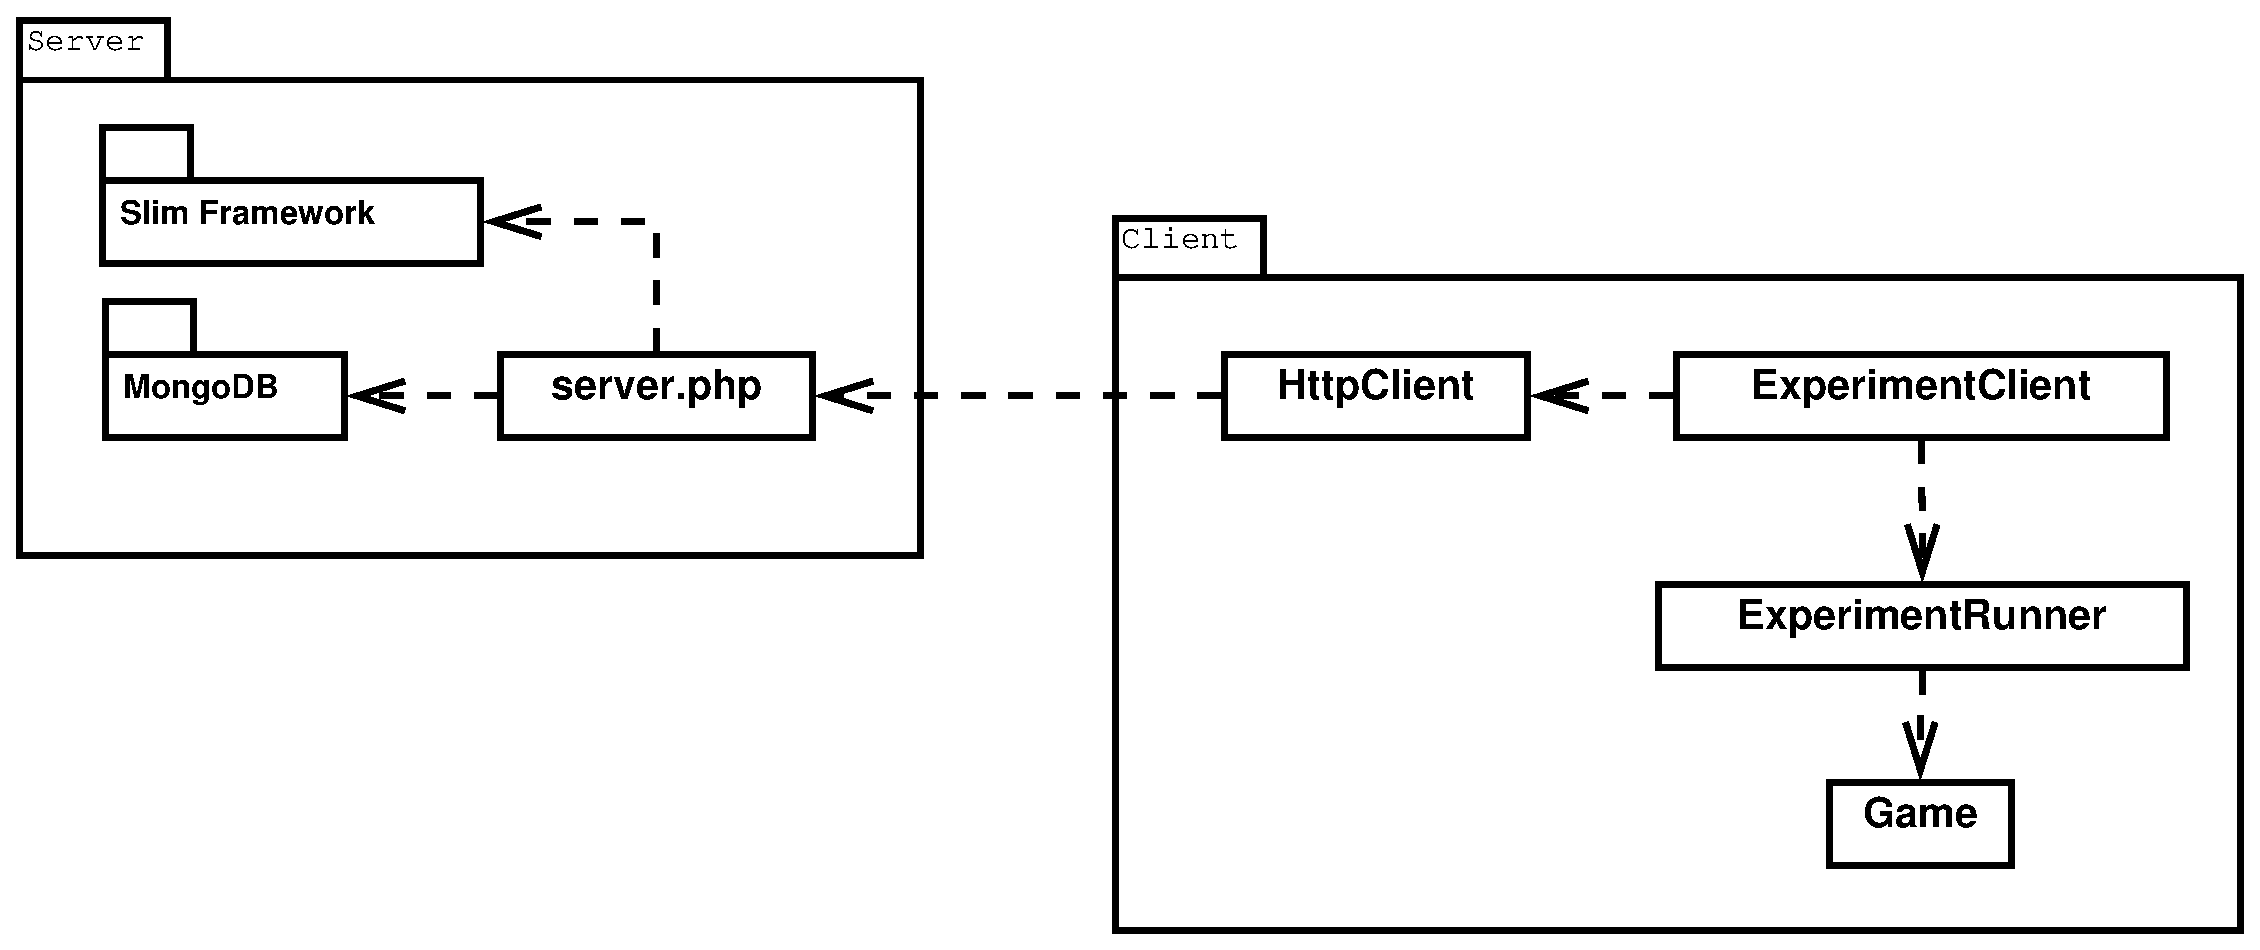
\includegraphics[width=\linewidth]{diagrams/testserver}
\caption{Test server structure}
\label{fig:testserver}
\end{figure}


The first two requirements suggest a client-server architecture.  A system was designed where experiments are stored in a MongoDB\footnote{MongoDB is an open source NoSQL database engine written in C++.  More details are available at \url{http://www.mongodb.org/about/introduction/}.} database with a PHP\footnote{PHP, a recursive acronym standing for `PHP: Hypertext Processor', is a popular open source scripting language used mainly for web development.  See \url{http://uk.php.net/manual/en/intro-whatis.php} for a quick introduction.} front end, which is accessed by a Java client class.  The client class connects to the server and asks for the next available experiment: as well as an ID for the experiment, it is provided with a JavaScript snippet specifying the parameters.  More specifically, the script is run in a scope where the fields of an instance of the Parameters class, and the Java packages containing the various classes that may need to be instantiated for the parameters, are available.  Running arbitrary JavaScript may be considered overkill, however due to the time constraints on the project, it was considered a superior solution to the alternative of defining some kind of serialisation language (either on top of XML or using custom mark up) to specify the parameters.  A typical script is shown in listing \ref{lst:typicalscript}---note how various objects are initialised with values fed into the constructors: this would require reasonably sophisticated markup language to achieve otherwise.  The experiment object is shown in figure \ref{fig:experiments}.

\begin{lstlisting}[breaklines=true,caption={A typical parameters script},captionpos=b,label=lst:typicalscript,float]
nodeExpansionThreshold = 30;
maximumSimulationLength = 100000;
pacManModel = new RandomNonRevPacMan();
ghostModel = new NeuralNetworkGhostController(new RouletteMoveSelectionStrategy(), 5, false);
tasks = [ ghostModel ];
selectionPolicy = new LevineUcbSelectionPolicy(4000);
opponent = new Legacy();
\end{lstlisting}

\begin{figure}
\centering
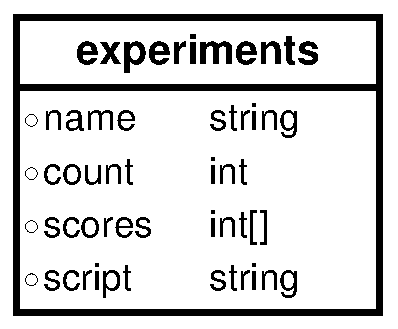
\includegraphics[scale=0.8]{diagrams/experiments}
\caption[The experiment object]{The experiment object.  The {\tt count} field starts off at the number of games that should be played with the parameters, and is decremented each time a client is given the experiment to run.  The {\tt scores} field holds the final scores for each of the games run.}
\label{fig:experiments}
\end{figure}

Several other choices were made to facilitate a quick implementation.  The chosen database system, MongoDB, is a NoSQL\footnote{NoSQL databases systems attempt to address some of the problems with traditional relational database systems (RDBMSs).  They are generally document-oriented, meaning arbitrary object graphs can be stored instead of highly structured data.  Interested readers can consult \url{http://en.wikipedia.org/wiki/NoSQL} for an overview.}, document-oriented database system which allows arbitrary denormalised object graphs to be stored.  Assuming the database server has already been installed, setup time is ostensibly nil: the program or programmer (by use of an interactive JavaScript console provided with the system) may simply start adding objects to a specified collection\footnote{A \emph{collection} is the rough equivalent of tables in a relational database system.  However, unlike tables, they do not have a precise schema, and two objects stored in the same collection may be completely different.} and a specified database name---if either of these do not exist, they are created.  By contrast, if using a system like MySQL, the programmer would have to set up the database with associated users and privileges, and execute lines upon lines of data definition language (DDL) code to create the tables.

Note also that a separate table would have to be created for the Scores field, as it is not possible to store an array of values in a SQL table.  There are ways around this---for example, one could store the scores as a comma-delimited list in a string ({\tt VARCHAR}) field, but this would greatly complicate the issue of performing numerical queries on the data.  However, the biggest issue is related to updating: if two clients finish at roughly the same time, they will both read the scores field to get its present value, add their own score to the end of the list, and save the new value.  Depending on the order of the operations, i.e., if both writes succeed both reads, one of the writes will be overwritten and the associated score will be lost.  The are also ways around this of course, but it starts to get complex here.  In contrast, MongoDB allows fields to contain arrays, and defines an atomic {\tt\$push} operator which adds a given element to an array.

The system makes use of MongoDB's {\tt findAndModify} operation, which updates the first document it finds matching the specified criteria and returns it, atomically.  This is useful when retrieving ``active'' experiments, that is, experiments for which the {\tt count} field has not yet been decremented to zero.  Since the sequence of actions ``search for experiment with count greater than zero'', ``decrement count'' and ``return experiment'' is executed atomically, concurrency is not an issue, and no two machines will think they are running the same experiment number.  This is also possible in SQL, but is arguably more complex.

PHP was chosen as the server-side language as it is quick to write simple websites in, and it was deemed that the rigour of a typed language was not necessary for this project.  It also allowed the Slim Framework\footnote{Slim is a ``micro framework'' for PHP that makes writing simple websites with routing logic easy.  It is online at \url{http://www.slimframework.com/}.} to be used, which facilitates URL routes for specific HTTP methods to be mapped to anonymous handler functions.  This choice of framework enabled the entire application to be implemented in three short functions in a single file.  This is included as appendix \ref{ap:server}; it is easy to read and understand in its entirety, and demonstrates that the system is indeed quick to implement.

\subsection{Protocol details}

Three routes are handled by the application, inspired by a REST style approach:

\begin{itemize}
\item {\tt GET /active\_experiment}: find an experiment with a count greater than zero, decrement that count, and return the experiment serialised as JSON\footnote{JSON (JavaScript Object Notation) is a data interchange language which is a subset of JavaScript.  It allows objects to be serialised in the form they would take if written as a JavaScript literal, thus for example, an array of integers is simply: {\tt [1, 2, 3, 4]}.  See \url{http://www.json.org} for more details.}.  If there are no such experiments, the {\tt HTTP 410 Gone} status code is returned instead.
\item {\tt POST /experiments/\$id}: saves a score to the experiment object with the specified ID.  The body of the request should contain the score to add, serialised as JSON.
\item {\tt POST /experiments}: saves an experiment to the collection of experiments.  The experiment to save should be included in the body of the request, serialised as JSON.
\end{itemize}

The Java client retrieves an experiment using the first route, runs the game, and when it has completed, saves the final score using the second route.  The third route was added for convenience to allow a small utility programme on the client to upload experiment scripts specified in files.




\chapter{Results and evaluation}
\label{ch:results}

\section{Overview}

The next section describes the method used to gather data on the effectiveness of the learning ghost controller, with the results being presented in Section \ref{sec:results}.  Section \ref{sec:overfitting} investigates the problem of overfitting, and the final section explores possible improvements to the base MCTS algorithm.

\section{Method}

The learning ghost controller described in Chapter \ref{ch:design} was successfully implemented in Java using the IntelliJ development environment, and a server to facilitate testing the project, detailed in Chapter \ref{ch:verification}, was developed.  The server makes it possible to specify a set of parameters for the algorithm in a JavaScript file, and allows any number of connected machines to run the games specified by the scripts and report back the final scores.

A number of these parameter scripts were created to investigate various aspects of the algorithm, and these will be detailed below.  Due to the high variance in the final scores for a given parameter set, 20 games were run for each script and an average was obtained for each set.  Reference will be made to whether results are ``statistically significant'': a result is taken to be significantly different from another if a Student's t-test on the two data sets gives $p < 0.05$.

The games were run over 12 identical computers each with 3.3~GHz Intel i5 processors and 4~Gb of memory.  Since the computers have four cores, each computer ran two instances of the experiment client: this meant each computer could run two games at once, halving the amount of time needed whilst saving resources and electricity.  The cluster ran up to 24 games simultaneously, and around 2000 games were run over a few days; this would have taken 1--2 weeks without the experiment server.

\section{Results}
\label{sec:results}

\subsection{Learning vs non-learning controller}

The first experiment aimed to assess broadly whether the learning ghost controller improved performance.  It was initially assumed that the agent would have poor performance if the learning controller started off with zero knowledge, so it was supplied with weights trained from data recorded in a game against the {\tt Legacy} controller.  Figure \ref{fig:results1} shows the average final scores obtained after playing 20 games using each of the six sample ghost controllers as opponents, first using {\tt Legacy} during playouts as a ``non-learning'' controller, and again using the learning controller.

\begin{figure}
\centering
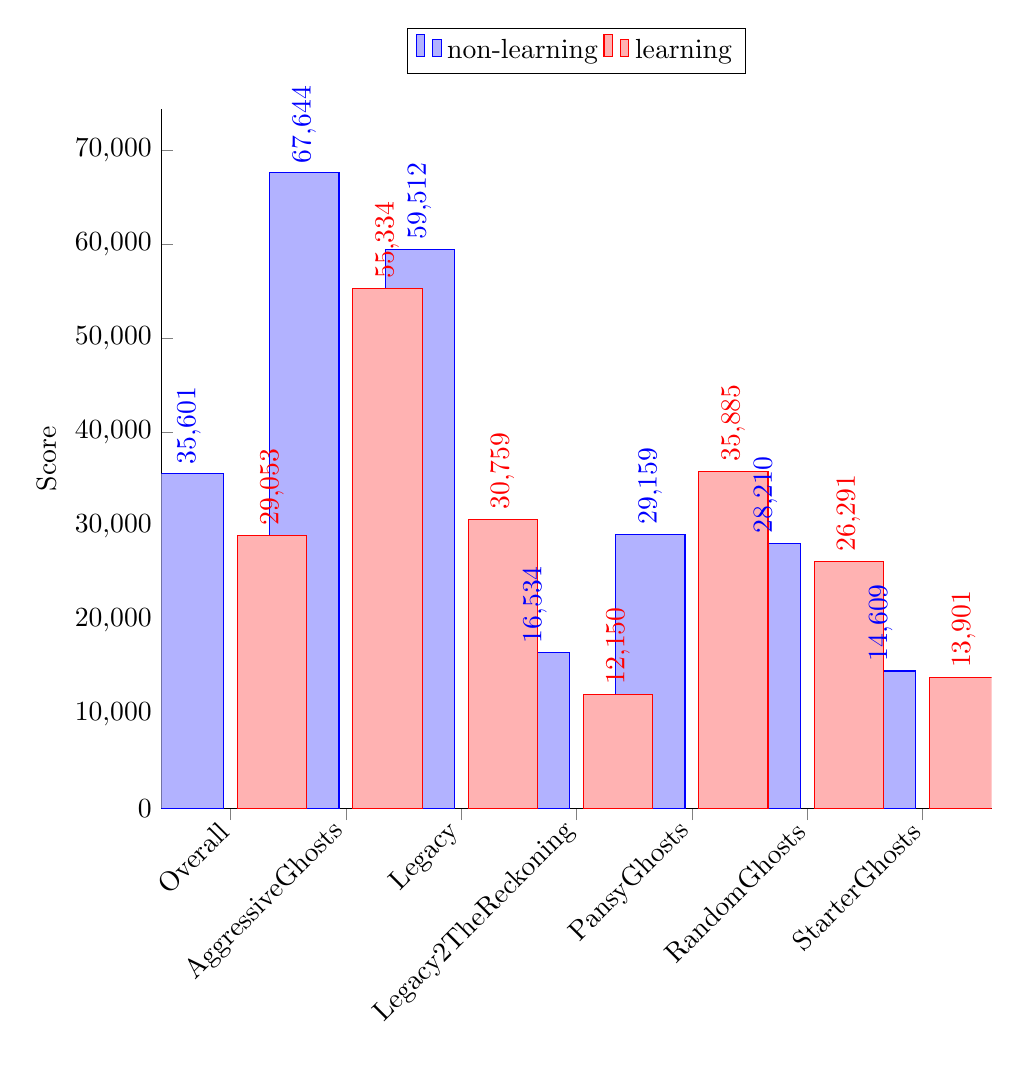
\begin{tikzpicture}
\pgfplotsset{every axis legend/.append style={
at={(0.5,1.05)},
anchor=south}}
\begin{axis}[
    %symbolic x coords={non-learning, learning},
    ybar = 5pt,
    symbolic x coords={Overall, AggressiveGhosts, Legacy, Legacy2TheReckoning, PansyGhosts, RandomGhosts, StarterGhosts},
    ylabel=Score,
    xtick=data,
    ymin=0,
    nodes near coords=\rotatebox{90}{\pgfmathprintnumber\pgfplotspointmeta},
    scaled y ticks=false,
    axis lines*=left,
    bar width=25pt,
    enlarge x limits=0.1,
    legend columns=4,
    width=\textwidth,
    x tick label style={rotate=45, anchor=east}
    ]
    
    \addplot coordinates {
       (Overall,35601)
       (AggressiveGhosts,67644)
       (Legacy,59512)
       (Legacy2TheReckoning,16534)
       (PansyGhosts,29159)
       (RandomGhosts,28210)
       (StarterGhosts,14609)
    };
    \addlegendentry{non-learning}
    
    \addplot coordinates {
       (Overall,29053)
       (AggressiveGhosts,55334)
       (Legacy,30759)
       (Legacy2TheReckoning,12150)
       (PansyGhosts,35885)
       (RandomGhosts,26291)
       (StarterGhosts,13901)
    };
    \addlegendentry{learning}
    
    
\end{axis}
\end{tikzpicture}
\caption[Learning vs non-learning ({\tt Legacy}) ghost controller]{Learning vs non-learning ({\tt Legacy}) ghost controller: averaged over all sample opponents, there is a decrease in performance when using the learning controller, but taking the {\tt PansyGhosts} controller on its own reveals an increase in performance.  Both results are statistically significant ($p < 0.05$).}
\label{fig:results1}
\end{figure}

\begin{figure}
\centering
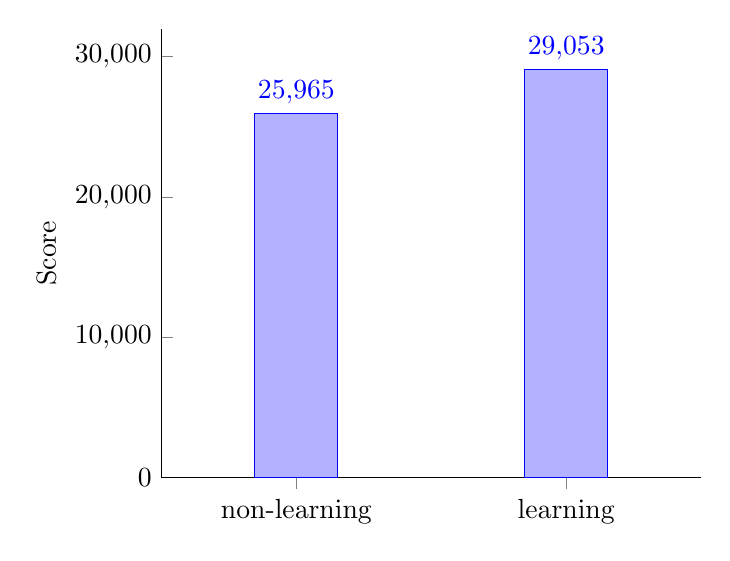
\begin{tikzpicture}
\pgfplotsset{every axis legend/.append style={
at={(0.5,-0.2)},
anchor=north}}
\begin{axis}[
    symbolic x coords={non-learning,learning},
    ylabel=Score,
    ybar=5pt,
    xtick=data,
    ymin=0,
    nodes near coords,
    scaled y ticks=false,
    axis lines*=left,
    bar width=30pt,
    enlarge x limits=0.5
    ]
    \addplot coordinates {
       (non-learning,25965)
       (learning,29053)
    };
\end{axis}
\end{tikzpicture}
\caption[Learning vs non-learning ({\tt RandomGhosts}) ghost controller]{Learning vs non-learning ({\tt RandomGhosts}) ghost controller: using the learning controller during rollouts shows slightly improved performance over using a random player, but not significantly so.}
\label{fig:resultsrandom}
\end{figure}

The results look at first glance disappointing, with the average over all 6 opponents being significantly lower when using the learning controller during playouts compared to using {\tt Legacy}; however, further investigation of the data revealed that performance against the {\tt PansyGhosts} controller showed a significant increase in performance as a result of using the learning controller.  Recall from Section \ref{sec:sampleghosts} that the {\tt PansyGhosts} controller causes all of the ghosts to always run away from Ms~Pac-Man, whilst the {\tt Legacy} controller causes three of the ghosts to always run towards Ms~Pac-Man: it would seem sensible that {\tt Legacy} would be a bad model for {\tt PansyGhosts} and thus the ability to learn the opposite behaviour of the opponent has clearly benefited the agent.  Figure \ref{fig:resultsrandom} shows that using the learning controller might be slightly better than using a random player, but the result is not statistically significant.

\subsection{Capping the rollout length}

It was conjectured that the reason for the lowered performance overall when using the learning controller is that time spent learning takes away from the time available to the MCTS algorithm, potentially leading to lower quality decisions.  Therefore the first experiment was repeated with the length of playouts (that is, the amount of \emph{game time} each playout is simulated for, not the length of time the simulation is run for) capped at 10 seconds, in the hope that the algorithm would be able to perform more playouts.  Figure \ref{fig:resultssr} shows that the learning controller still gives a decreased performance; in retrospect, the 10 second cap may still have been too high to really effect the outcome.

\begin{figure}
\centering
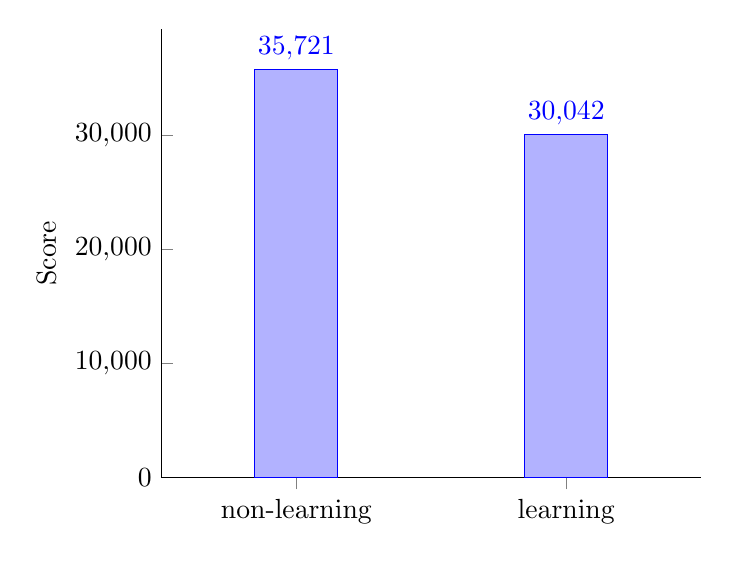
\begin{tikzpicture}
\pgfplotsset{every axis legend/.append style={
at={(0.5,-0.2)},
anchor=north}}
\begin{axis}[
    symbolic x coords={non-learning,learning},
    ylabel=Score,
    ybar=5pt,
    xtick=data,
    ymin=0,
    nodes near coords,
    scaled y ticks=false,
    axis lines*=left,
    bar width=30pt,
    enlarge x limits=0.5
    ]
    \addplot coordinates {
       (non-learning,35721)
       (learning,30042)
    };
\end{axis}
\end{tikzpicture}
\caption[Learning with a 10 second maximum rollout length]{Learning with a 10 second maximum rollout length: capping the rollout length at 10 seconds does not seem to alter the results much as they still show a decrease in performance when using the learning controller.}
\label{fig:resultssr}
\end{figure}

\subsection{Non-real-time learning}

In order to properly exclude the possibility that the time spent learning decreases the quality of the MCTS results, the first experiment was repeated; instead of running in real-time however, every decision was given exactly 1000 iterations of MCTS and the ghost neural networks were trained for exactly 100 iterations on every ghost decision observed.  The results in Figure \ref{fig:resultsrealtime} still show a decrease in overall performance when using the learning controller during playouts, but it is not a statistically significant difference.  The {\tt PansyGhosts} controller still shows a significant increase in performance.  It is not clear why the learning controller should not be at least as good as using {\tt Legacy} during playouts when the number of iterations of MCTS is fixed.

\begin{figure}
\centering
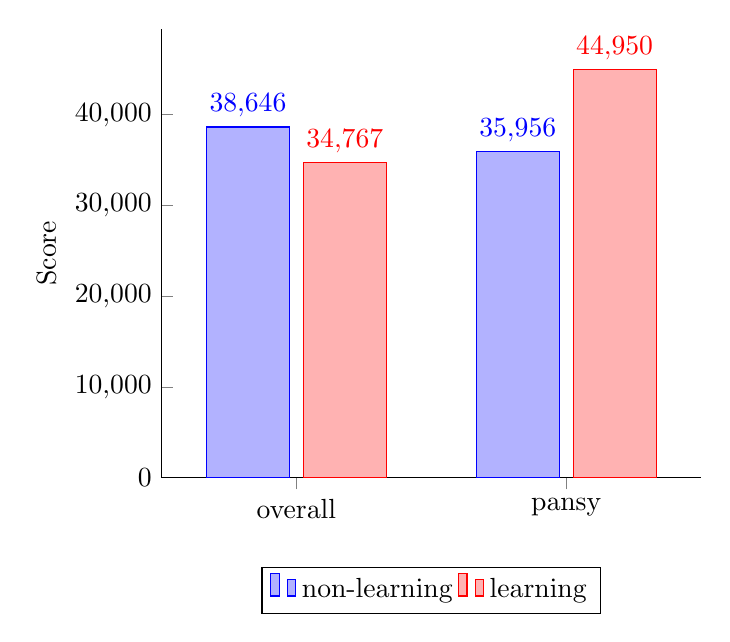
\begin{tikzpicture}
\pgfplotsset{every axis legend/.append style={
at={(0.5,-0.2)},
anchor=north}}
\begin{axis}[
    symbolic x coords={overall,pansy},
    ylabel=Score,
    ybar=5pt,
    xtick=data,
    ymin=0,
    nodes near coords,
    scaled y ticks=false,
    axis lines*=left,
    bar width=30pt,
    enlarge x limits=0.5,
    legend columns=4
    ]
    \addplot coordinates {
       (overall,38646)
       (pansy,35956)
    };
    \addlegendentry{non-learning}
    
    \addplot coordinates {
       (overall,34767)
       (pansy,44950)
    };
    \addlegendentry{learning}
\end{axis}
\end{tikzpicture}
\caption[Non-realtime learning]{Non-realtime learning: when every decision is given exactly 1000 iterations of MCTS and the ghost networks are trained exactly 100 times for every new example, the learning controller still fares slightly worse overall, but the result is not statistically significant.  On the other hand, {\tt PansyGhosts} taken on its own shows a statistically significant improvement with learning.}
\label{fig:resultsrealtime}
\end{figure}


\subsection{The effect of seeding the neural network}

The experiments described so far have used the learning controller initiated with weights trained from data recorded in a game against {\tt Legacy} (i.e., the controller should start off behaving like {\tt Legacy}).  This is because it was initially assumed that the agent would do really poorly to start off with until the ghost controller learned some behaviour, and that it may never get the chance to learn behaviour if the agent died early on as a result of poor decisions.  It was decided to verify this belief, and so 20 games were run against all 6 opponent controllers for each of the following four cases: real-time with and without pre-trained weights, and non-real-time with and without pre-trained weights.  The results are shown in Figure \ref{fig:resultsuntrained}, and they are somewhat surprising: using pre-trained weights confers no advantage.  It is conjectured that the ghost behaviour is actually rather easy to learn, and that it does not take long for this to happen.

\begin{figure}
\centering
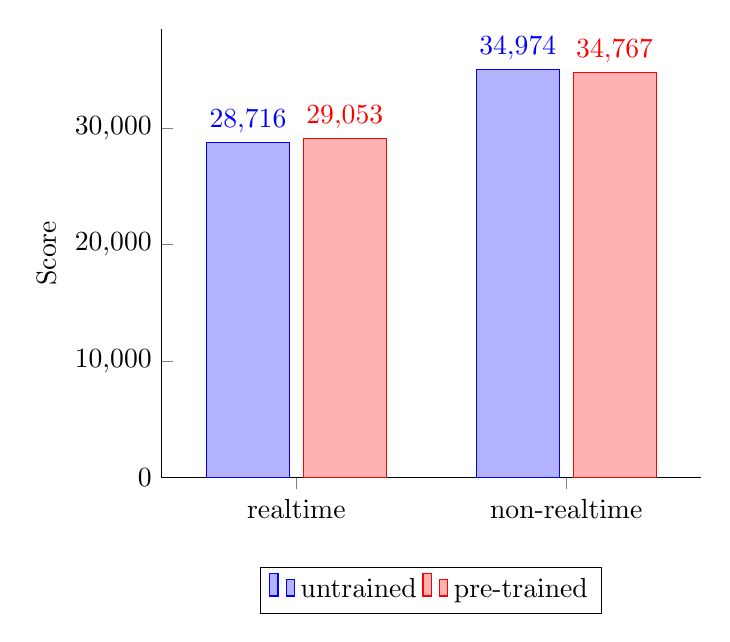
\begin{tikzpicture}
\pgfplotsset{every axis legend/.append style={
at={(0.5,-0.2)},
anchor=north}}
\begin{axis}[
    symbolic x coords={realtime,non-realtime},
    ylabel=Score,
    ybar=5pt,
    xtick=data,
    ymin=0,
    nodes near coords,
    scaled y ticks=false,
    axis lines*=left,
    bar width=30pt,
    enlarge x limits=0.5,
    legend columns=4
    ]
    \addplot coordinates {
       (realtime,28716)
       (non-realtime,34974)
    };
    \addlegendentry{untrained}
    
    \addplot coordinates {
       (realtime,29053)
       (non-realtime,34767)
    };
    \addlegendentry{pre-trained}
\end{axis}
\end{tikzpicture}
\caption[Untrained vs pretrained]{Untrained vs pretrained: supplying the learning controller with weights trained from {\tt Legacy} to start from confers no significant advantage, either in realtime or not.}
\label{fig:resultsuntrained}
\end{figure}


\subsection{The effect of varying the number of training iterations}

\begin{figure}
\centering
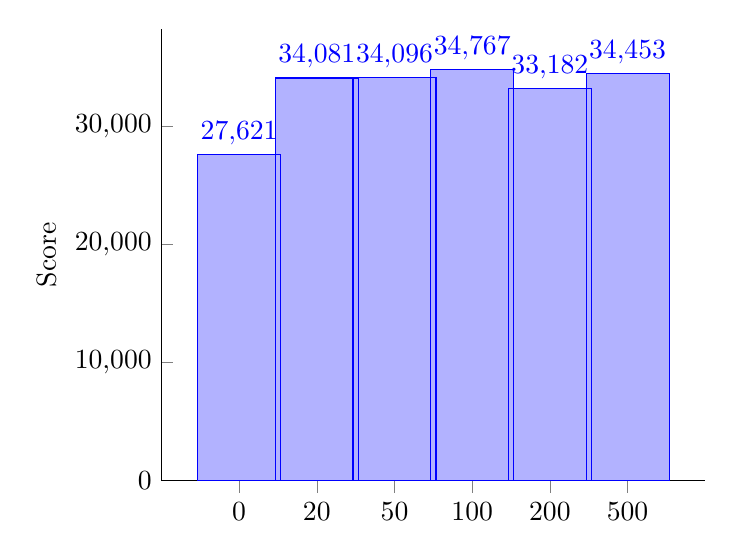
\begin{tikzpicture}
\pgfplotsset{every axis legend/.append style={
at={(0.5,-0.2)},
anchor=north}}
\begin{axis}[
    symbolic x coords={0,20,50,100,200,500},
    ylabel=Score,
    ybar=40pt,
    xtick=data,
    ymin=0,
    nodes near coords,
    scaled y ticks=false,
    axis lines*=left,
    bar width=30pt,
    enlarge x limits=0.2,
    width=0.7\textwidth
    ]
    \addplot coordinates {
       (0,27621)
       (20,34081)
       (50,34096)
       (100,34767)
       (200,33182)
       (500,34453)
    };
\end{axis}
\end{tikzpicture}
\caption[The effect of varying the number of training iterations]{The effect of varying the number of training iterations: there is no significant difference between any of the values, but 0 iterations gives noticeably lowered performance.}
\label{fig:resultsiterations}
\end{figure}


A series of experiments were run in non-real-time mode to investigate the effect of changing the number of iterations each new observed training example was learned over.  20 games were played against each of the 6 opponents, for each of the following iteration counts: 0, 20, 50, 100, 200 and 500.  In all cases except the first, the number of iterations of MCTS run was 1000.  Figure \ref{fig:resultsiterations} shows the results: varying the number of iterations of training does not alter the average final score achieved.  This lends further evidence to the conjecture that the ghost behaviour is particularly trivial for the network to learn, but shows that something is being learned at the start.


\subsection{The effect of move selection strategy}

\begin{figure}
\centering
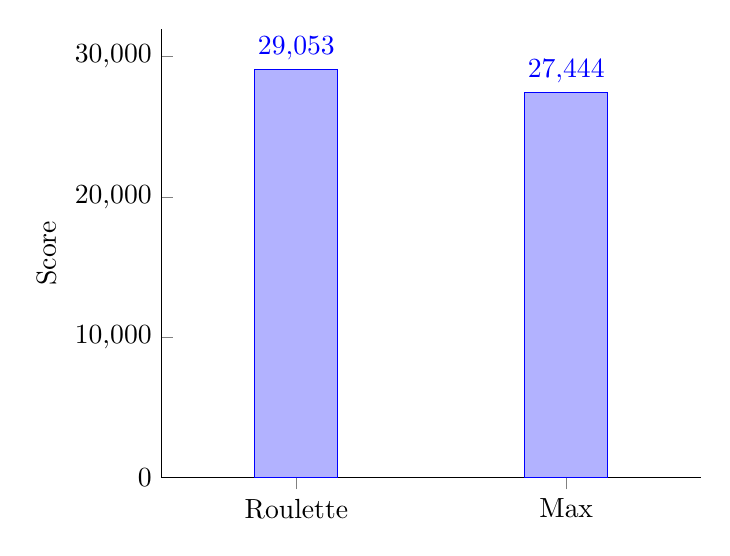
\begin{tikzpicture}
\pgfplotsset{every axis legend/.append style={
at={(0.5,-0.2)},
anchor=north}}
\begin{axis}[
    symbolic x coords={Roulette, Max},
    ylabel=Score,
    ybar=35pt,
    xtick=data,
    ymin=0,
    nodes near coords,
    scaled y ticks=false,
    axis lines*=left,
    bar width=30pt,
    enlarge x limits=0.5,
    ]
    \addplot coordinates {
       (Roulette,29053)
       (Max,27444)
    };
\end{axis}
\end{tikzpicture}
\caption[Roulette vs maximum move selection]{Roulette vs maximum move selection: using roulette selection is mariginally better than using maximum, but the result is not statistically significant.}
\label{fig:resultsmax}
\end{figure}

A final experiment was run to investigate the effect of the move selection strategy.  Recall from Section \ref{sec:nnalgorithm} the two ways of selecting a move from the neural network output: all the experiments described so far have used the {\tt RouletteSelectionStrategy} class, which selects a move with a probability proportional to its respective output.  This seems like a good strategy since Monte Carlo tree search is a probabilistic algorithm, and it would presumably help the performance if even unlikely game states are explored from time to time in case they are realised.  This hypothesis was verified by running 20 games using the learning controller in playouts against each of the 6 ghost teams, once using roulette selection and once using maximum selection.  The results are shown in Figure \ref{fig:resultsmax}: roulette selection does indeed appear to be slightly better than maximum selection, but again the result is not statistically significant.

\subsection{Statistical significance}

Lastly, a note on statistical significance.  Many of the results presented here are not statistically significant---the final scores obtained from the game for each experiment run have a high level of variance, as subtly different choices in each game can result in drastic differences in score, making it difficult to draw strong conclusions.  This could be ameliorated by running substantially more games, as 20 may not have been enough due to the high variance, but the time constraints of the project limited the total number of games that could be run.

\section{The problem of overfitting}
\label{sec:overfitting}

Overfitting is a problem where a learning algorithm can classify the training set really well, but is unable to generalise well.  The neural networks in the project were verified against the same data as they were trained with---it was realised towards the end of the project that this could be a source of error in the reported results, so it was decided to investigate the issue.  Two games were recorded for every ghost team and in the first case, the neural networks were trained and verified with the same data; in the second, they were trained with data from one game and verified with the data from the other recorded game.  By verified, it is meant that the neural network was allowed to make a prediction for each of the rows of data, and the prediction was checked against the actual output; the number of wrong predictions out of the total number of rows of data gives an error percentage.

The results are shown in Figure \ref{fig:resultsclasserror}: the reported error is much higher when a diffent data set is used for verification, so overfitting is an issue.  There are various ways to mitigate this, such as training on more examples, or using a better algorithm more immune to overfitting.  It could also be that the inputs to the neural network were poorly chosen.  For example, rather than feeding the next direction towards and away from Ms~Pac-Man as inputs and outputting a direction, the network could instead output a value which makes the choice to go towards or away.

Another interesting result shown in the graph is that the {\tt PansyGhosts} controller has a very low error, but it is not clear why this is the case.  It is a completely deterministic model, but so is {\tt AggressiveGhosts} for example, which has a much higher error.  It may have to do with the fact that two different distance measurements are used for chasing Pac-Man, and only one for running away, but more investigation is clearly warranted into this result.

\begin{figure}
\centering
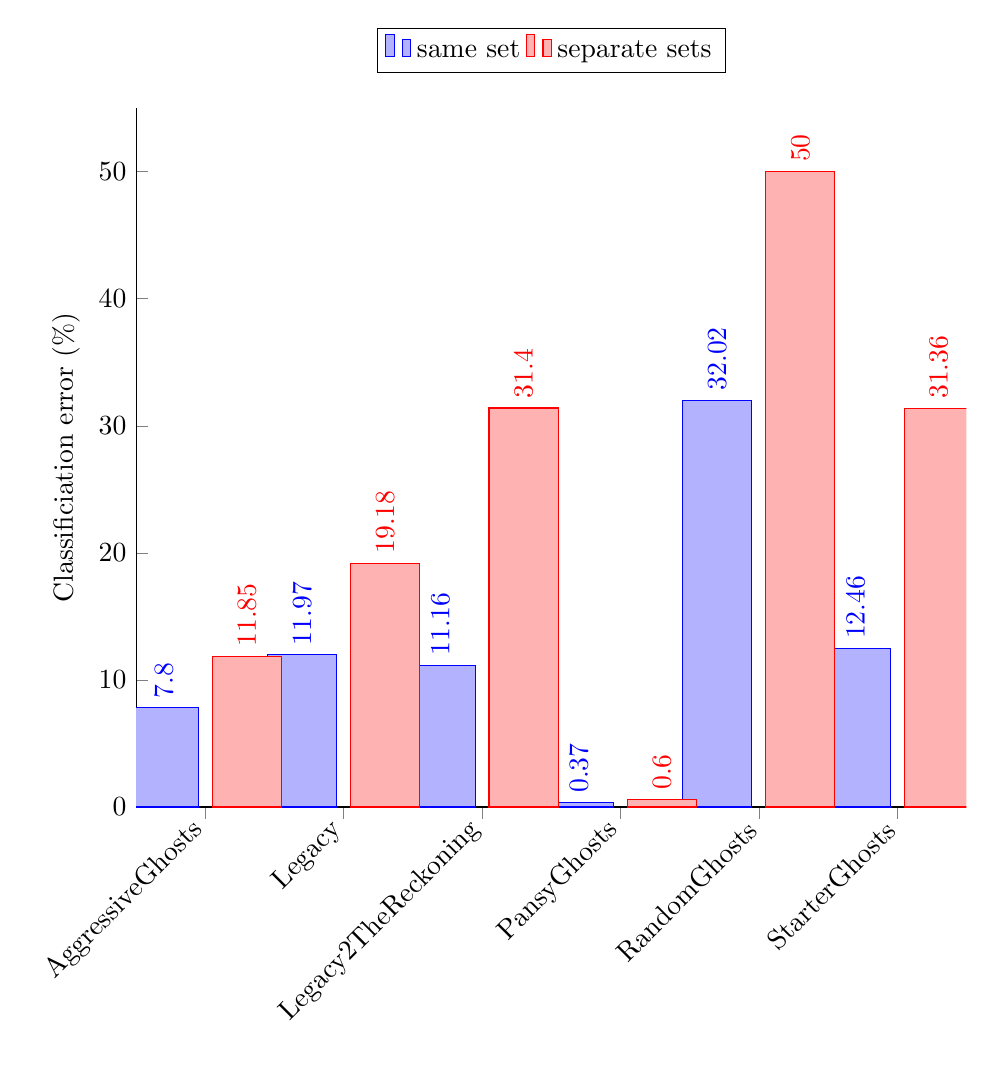
\begin{tikzpicture}
\pgfplotsset{every axis legend/.append style={
at={(0.5,1.05)},
anchor=south}}
\begin{axis}[
    ybar=5pt,
    symbolic x coords={AggressiveGhosts, Legacy, Legacy2TheReckoning, PansyGhosts, RandomGhosts, StarterGhosts},
    ylabel=Classificiation error (\%),
    xtick=data,
    ymin=0,
    nodes near coords=\rotatebox{90}{\pgfmathprintnumber\pgfplotspointmeta},
    scaled y ticks=false,
    axis lines*=left,
    bar width=25pt,
    enlarge x limits=0.1,
    legend columns=4,
    width=\textwidth,
    x tick label style={rotate=45, anchor=east}
    ]
    
    \addplot coordinates {
        (AggressiveGhosts,7.80)
        (Legacy,11.97)
        (Legacy2TheReckoning,11.16)
        (PansyGhosts,0.37)
        (RandomGhosts,32.02)
        (StarterGhosts,12.46)
    };
    \addlegendentry{same set}
    
    \addplot coordinates {
        (AggressiveGhosts,11.85)
        (Legacy,19.18)
        (Legacy2TheReckoning,31.4)
        (PansyGhosts,0.6)
        (RandomGhosts,50)
        (StarterGhosts,31.36)
    };
    \addlegendentry{separate sets}
\end{axis}
\end{tikzpicture}
\caption[Classification error when learning different ghost models]{Classification error when learning different ghost models: the error is shown for two cases, the first where the same set was used for training and verification, and the second where two different sets were used for training and validation in each case.}
\label{fig:resultsclasserror}
\end{figure}


\section{Ideas for improving the base MCTS algorithm}
\label{sec:maastricht}

The current best plain MCTS agents are better than the agent used in this project, achieving significantly higher scores.  A particularly good example is the ``maastricht'' agent developed by \citep{Pepels2012}.  This agent has various differences in its algorithms which may contribute to its greater success---it was intended to trial these potential improvements on the agent used in this project, but there was not enough time.  The differences are summarised here for reference and potential future work.

First of all, nodes represetning a reversal in direction for Ms~Pac-Man are not considered past the first layer on the tree.  The agent in this work can consider a potentially infinite sequence of reversals, taking up a lot of processing time and not contributing much knowledge to the tree.

Similar to the agent described by \cite{Ikehata2011}, the agent operates in one of three states: \emph{Ghost score}, \emph{Pill score}, and \emph{survival}. This enables the agent to change its behaviour depending on local conditions, such as whether or not a ghost is nearby.  The algorithm also encodes some long term goals to help bring the agent closer to scoring opportunities that can be missed by the MCTS algorithm.

If during the selection phase Ms~Pac-Man loses a life, the playout phase is re-started from the last visited junction.  If Ms~Pac-Man eats a ghost or power pill during the selction phase, the rollout is started immediately, as the ghost state is unpredictable.  The depth of the tree is limited to only include nodes a certain predefined distance from the agent's current location.  This may increase the space explored, and there is not much point simulating very far into the future due to the non-determinism of the ghosts.

The playouts during the simulation phase have different stopping conditions: their agent stops the playout if Ms~Pac-Man loses a life, a certain number of ticks have passed, the next level is reached, or Ms~Pac-Man eats a power pill while a previous power pill is active.  The latter is included to act as a punishment for making this poor choice.




\chapter{Summary and conclusions}
\label{ch:summary}

\section{Summary}
An existing agent for Ms~Pac-Man utilising Monte Carlo tree search was augmented by adding a ghost controller to use during MCTS playouts that is capable of learning its behaviour from the opponent ghost team by using neural networks.  In order to evaluate the additions, an ``experiment server'' was created to allow experiments to be specified in JavaScript files and farmed out to many computers to be executed concurrently.

A total of 1900 games were run using the server to investigate the effect of changing various parameters in the algorithm.  The experiment server was a definite success, allowing these games to be run over a few days rather than the week or two it would have otherwise taken.  The success of the learning ghost controller is summarised in the following section.

\section{Conclusions}

As shown in chapter \ref{ch:results}, using the learning controller during playouts instead of a non-learning controller such as {\tt Legacy} appears to decrease the performance of the original agent when averaged over all of the sample ghost controllers in the framework.  However, the framework ghost teams are reasonably similar for the most part, and using the {\tt Legacy} controller during playouts gives reasonable results.

On the other hand, the {\tt PansyGhosts} controller is almost exactly opposite to {\tt Legacy} in that it always runs away from Ms~Pac-Man rather than always running towards her, and using the learning controller during playouts against this team shows a significant improvement in the score over using {\tt Legacy} in the playouts.  It is clear therefore that the controller is able to learn the behaviour of the opponent, which gives an advantage when the opponent is drastically different from {\tt Legacy}.

The results also indicate that the ghost behaviour is particularly easy to learn.  This suggests that neural networks may not have been the best choice, and that some other form of simpler learning would have been better.

\section{Further work}

The performance of the original agent falls short of other current agents using plain Monte Carlo tree search: it would be prudent to investigate the reasons for this and attempt to bring the ``vanilla'' agent to the same level of performance as its contemporaries.

Further investigation is required to understand why the performance of the learning agent is not even as good as the original agent when playing against most of the framework ghosts.  The agent should also be evaluated against better ghost teams as the ones used are very basic and quite similar in most cases.

Finally, using neural networks may not have been the best choice for this project and other machine learning techniques could be investigated.  Section \ref{sec:alternativetreatments} gives several suggestions, such as using a classification algorithm or reinforcement learning.


%no vertical spacing before appendix headings
\titlespacing*{\chapter}{0pt}{0pt}{40pt}

\bibliography{thesis}

\chapter{Outline project specification}
\label{ap:outlinespec}
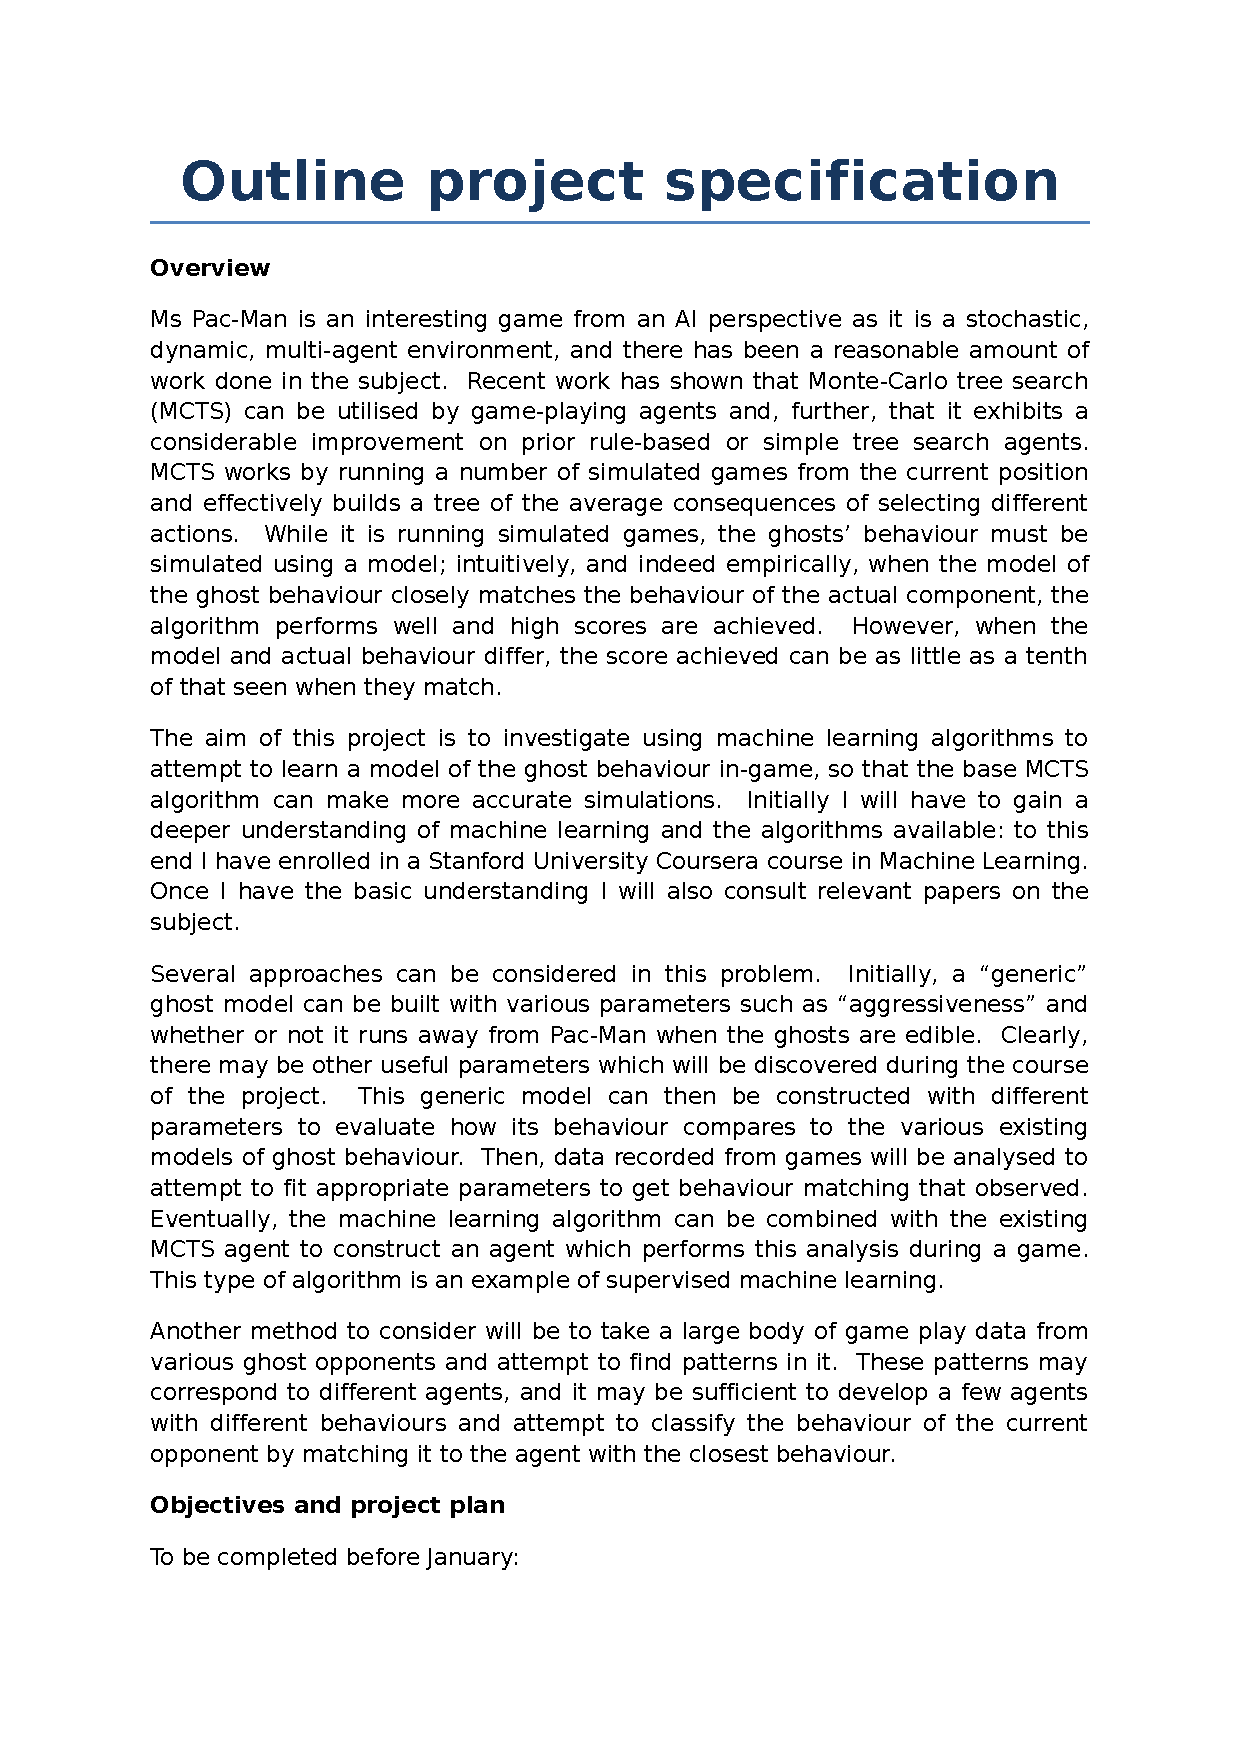
\includepdf[pages=-]{diagrams/outlinespec.pdf}

\chapter{Server source listing}
\label{ap:server}
\lstinputlisting[language=PHP,caption={server/server.php}]{../server/server.php}

\chapter{MATLAB neural network implementation}
\label{ap:matlab}
\lstinputlisting[language=Octave,caption={matlab/nntrain.m}]{../matlab/nntrain.m}
\lstinputlisting[language=Octave,caption={matlab/sig.m}]{../matlab/sig.m}
\lstinputlisting[language=Octave,caption={matlab/sigd.m}]{../matlab/sigd.m}

\chapter{User guide}
\label{ch:userguide}




\chapter{Program listing}
\label{ap:listing}

\end{document}
